% ============================================================
%  Comparativa.tex
%  Synthetic Difference-in-Differences: Python vs Stata
%  Dataset: Cigar (Baltagi, 2002) -- 46 estados, 1963-1992
% ============================================================
\documentclass[11pt, a4paper]{article}

\usepackage[utf8]{inputenc}
\usepackage[T1]{fontenc}
\usepackage[margin=2.5cm]{geometry}
\usepackage{booktabs}
\usepackage{graphicx}
\usepackage{subcaption}
\usepackage{caption}
\usepackage{float}
\usepackage{amsmath}
\usepackage{array}
\usepackage{xcolor}
\usepackage{colortbl}
\usepackage{multirow}
\usepackage{hyperref}
\usepackage{lmodern}
\usepackage{microtype}
\usepackage{parskip}

\hypersetup{colorlinks=true, linkcolor=blue!60!black, urlcolor=blue!60!black}

\definecolor{pyblue}{RGB}{31,119,180}
\definecolor{stgreen}{RGB}{44,160,44}
\definecolor{matchrow}{RGB}{220,255,220}
\definecolor{headgray}{RGB}{235,235,235}

\newcommand{\py}{\textcolor{pyblue}{\textbf{Python}}}
\newcommand{\st}{\textcolor{stgreen}{\textbf{Stata}}}
\newcommand{\pmark}{\textcolor{pyblue}{$\bullet$}}
\newcommand{\smark}{\textcolor{stgreen}{$\bullet$}}

% Significance stars
\newcommand{\sigone}{$^{***}$}
\newcommand{\sigtwo}{$^{**}$}
\newcommand{\sigthree}{$^{*}$}

\captionsetup{font=small, labelfont=bf}

% ============================================================
\begin{document}

\begin{titlepage}
  \centering
  \vspace*{3cm}
  {\LARGE\bfseries Comparativa: Synthetic Difference-in-Differences\\[0.4em]
  \py{} (\texttt{synthdid.py}) vs \st{} (\texttt{sdid})\\[1em]}
  {\large Dataset Cigar (Baltagi, 2002) --- Experimentos con diferentes configuraciones}\\[2em]
  {\normalsize
    \textbf{Datos:} 46 estados de EE.UU., 1963--1992 $\cdot$ \textit{Outcome:} ventas de cigarrillos (paquetes per c\'apita)\\[0.3em]
    \textbf{Tratamiento:} alzas idiosincrásicas del precio real $>10\%$ (proxy de alzas fiscales), adopción escalonada 1975--1986\\[0.3em]
    \textbf{Cohortes:} 8 estados tratados en 7 años de adopción distintos\\[2em]
  }
  {\small
    \begin{tabular}{ll}
      \toprule
      \textbf{Paquete} & \textbf{Referencia} \\
      \midrule
      \py{} \texttt{synthdid.py} & Este repositorio (basado en Arkhangelsky et al., 2021) \\
      \st{} \texttt{sdid} & Pailañir \& Clarke (2022), SSC \\
      \bottomrule
    \end{tabular}
  }
  \vfill
  {\small Marzo 2026}
\end{titlepage}

\tableofcontents
\newpage

% ============================================================
\section{Descripción del Experimento}
% ============================================================

\subsection*{Dataset y Variable de Tratamiento}

El dataset \textit{Cigar} contiene datos de panel de 46 estados de EE.UU. para los años 1963--1992 ($N=46$, $T=30$). La variable de resultado es \texttt{sales} (paquetes de cigarrillos per c\'apita). El precio real se deflact\'o usando el CPI y se construy\'o una variable de tratamiento \textbf{escalonado} identificando los estados que experimentaron un alza idiosincrásica del precio real $>10\%$ en un solo año respecto a la tendencia nacional (proxy de un alza fiscal estatal).

\begin{table}[H]
\centering
\caption{Estados tratados y año de adopción}
\begin{tabular}{ccc}
\toprule
Estado & Año adopción & Alza real (\%) \\
\midrule
3  & 1975 & 13.8 \\
9  & 1976 & 13.4 \\
40 & 1976 & 10.1 \\
15 & 1978 & 11.8 \\
49 & 1979 & 10.2 \\
7  & 1981 & 13.2 \\
23 & 1983 & 12.7 \\
42 & 1986 & 10.8 \\
\bottomrule
\end{tabular}
\end{table}

\subsection*{Configuración base de ambos paquetes}

\begin{center}
\begin{tabular}{lll}
\toprule
Parámetro & \py{} & \st{} \\
\midrule
Regularización SDID & $\zeta_\omega = \eta \cdot \hat{\sigma}$, $\eta=(N_1 T_1)^{1/4}$ & Idem \\
Regularización SC   & $\zeta_\omega = 10^{-6} \cdot \hat{\sigma}$ & Idem \\
Pesos SC lambda     & $\lambda = \mathbf{0}$ (sin ponderación pre-periodo) & Idem \\
Covariables (projected) & OLS con todas las dummies + pseudoinversa & Idem \\
Optimizador & Frank-Wolfe & Frank-Wolfe \\
SE por defecto & Placebo (sin reemplazo) & Placebo \\
Réplicas (base) & 100 & 50 \\
Semilla & 42 & 42 \\
\bottomrule
\end{tabular}
\end{center}

% ============================================================
\newpage
\section{Experimento 1: Estimación SDID Base}
% ============================================================

Estimación del ATT global y por cohorte usando el estimador SDID con errores estándar \textbf{placebo} (100 réplicas).

\subsection{Resultado Global}

\begin{table}[H]
\centering
\caption{SDID --- ATT global (SE Placebo, 100 réplicas, semilla=42)}
\begin{tabular}{lcccc}
\toprule
\textbf{Paquete} & \textbf{ATT} & \textbf{SE} & \textbf{t} & \textbf{p-valor} \\
\midrule
\rowcolor{headgray}
\py{} \texttt{synthdid.py} & $-13.8505$ & $5.2864$ & $-2.6200$ & $0.0088^{***}$ \\
\st{} \texttt{sdid}         & $-13.8505$ & $5.3062$ & $-2.61$   & $0.009^{***}$ \\
\midrule
\multicolumn{2}{l}{\textit{Diferencia absoluta ATT}} & \multicolumn{3}{r}{$0.0000$} \\
\multicolumn{2}{l}{\textit{Diferencia SE}} & \multicolumn{3}{r}{$0.0198$ \textcolor{gray}{(diferencia residual por RNG)}} \\
\bottomrule
\end{tabular}\\[0.4em]
{\small \textbf{Nota:} Los ATT son numéricamente idénticos. La diferencia en SE se debe \textit{únicamente} al generador de números aleatorios (RNG): Stata usa \texttt{mt64} (Mersenne Twister 64-bit) mientras que NumPy usa \texttt{MT19937}; con la misma semilla producen secuencias distintas. Con suficientes réplicas ($\gtrsim$500) ambos convergen al mismo valor asintótico.}
\end{table}

\subsection{ATT por Cohorte de Adopción}

\begin{table}[H]
\centering
\caption{ATT por cohorte (\py{} \texttt{synthdid.py})}
\begin{tabular}{cccccccc}
\toprule
Año & ATT cohorte & Peso ($w_k$) & $N_0$ & $T_0$ & $N_1$ & $T_1$ \\
\midrule
1975 & $-13.5634$ & $0.1636$ & 38 & 12 & 1 & 18 \\
1976 & $-30.6843$ & $0.3091$ & 38 & 13 & 2 & 17 \\
1978 & $-14.9199$ & $0.1364$ & 38 & 15 & 1 & 15 \\
1979 & $ -2.9917$ & $0.1273$ & 38 & 16 & 1 & 14 \\
1981 & $ -0.2916$ & $0.1091$ & 38 & 18 & 1 & 12 \\
1983 & $  3.5590$ & $0.0909$ & 38 & 20 & 1 & 10 \\
1986 & $ -0.3653$ & $0.0636$ & 38 & 23 & 1 &  7 \\
\midrule
\textbf{Global} & $\mathbf{-13.8505}$ & $1.0000$ & & & & \\
\bottomrule
\end{tabular}\\[0.4em]
{\small $N_0$: unidades de control, $T_0$: periodos pre-tratamiento, $N_1$: tratados, $T_1$: post-tratamiento.}
\end{table}

% ============================================================
\newpage
\section{Experimento 2: Comparación de Métodos SDID vs SC vs DiD}
% ============================================================

Se comparan los tres estimadores disponibles en ambos paquetes bajo el mismo SE placebo.

\begin{table}[H]
\centering
\caption{Comparación SDID vs SC vs DiD --- SE Placebo (100 reps, semilla=42)}
\setlength{\tabcolsep}{5pt}
\begin{tabular}{llcccc}
\toprule
& \textbf{Método} & \textbf{ATT} & \textbf{SE} & \textbf{t} & \textbf{p-valor} \\
\midrule
\multirow{3}{*}{\py{}}
  & SDID & $-13.8505$ & $5.2864$ & $-2.6200$ & $0.0088^{***}$ \\
  & SC   & $-13.3720$ & $5.2864$ & $-2.5295$ & $0.0114^{**}$ \\
  & DiD  & $-19.4820$ & $5.2864$ & $-3.6853$ & $0.0002^{***}$ \\
\midrule
\multirow{3}{*}{\st{}}
  & SDID & $-13.8505$ & $5.3062$ & $-2.61$ & $0.009^{***}$ \\
  & SC   & $-13.3721$ & $4.6632$ & $-2.87$ & $0.004^{***}$ \\
  & DiD  & $-19.4820$ & $6.8815$ & $-2.83$ & $0.005^{***}$ \\
\midrule
\multirow{3}{*}{\textit{Dif.}}
  & SDID & $0.0000$ & \cellcolor{matchrow}$\mathbf{0.0198}$ & & \\
  & SC   & \cellcolor{matchrow}$\mathbf{0.0001}$ & $0.6232$ & & \\
  & DiD  & $0.0000$ & $-1.5951$ & & \\
\bottomrule
\end{tabular}\\[0.4em]
{\small \textbf{Nota:} Los ATT son numéricamente idénticos entre paquetes para todos los métodos. Las diferencias en SE son debidas \textit{exclusivamente} al RNG (\texttt{mt64} en Stata vs \texttt{MT19937} en NumPy): con la misma semilla, cada implementación extrae permutaciones distintas. Con $\gtrsim$500 réplicas ambos convergen al mismo SE asintótico.}
\end{table}

\subsection*{Interpretación}

\begin{itemize}
  \item \textbf{SDID, SC y DiD:} Los ATT son numéricamente idénticos entre paquetes. La única diferencia residual está en el SE, causada por el RNG (\texttt{mt64} en Stata vs \texttt{MT19937} en NumPy): con la misma semilla extraen permutaciones distintas. Con $\gtrsim$500 réplicas ambos convergen al mismo SE verdadero.
  \item \textbf{SC:} La diferencia en ATT es de $0.0001$ (essencialmente cero). Ambas implementaciones usan $\zeta_\omega = 10^{-6} \cdot \hat\sigma$, sin ponderación pre-periodo ($\lambda = \mathbf{0}$) y sin centrado por media.
  \item \textbf{Conclusión:} SDID es el estimador más robusto y consistente entre implementaciones; SC y DiD también producen resultados idénticos.
\end{itemize}

% ============================================================
\newpage
\section{Experimento 3: Métodos de Inferencia}
% ============================================================

Se comparan tres métodos de cálculo de errores estándar para el estimador SDID: \textbf{Placebo}, \textbf{Bootstrap} y \textbf{Jackknife}. El ATT es idéntico en todos los casos (determinístico); solo cambia el SE.

\begin{table}[H]
\centering
\caption{SDID --- Comparación de métodos de inferencia (semilla=42, 100 reps para Placebo/Bootstrap)}
\begin{tabular}{llccccc}
\toprule
\textbf{Paquete} & \textbf{Método SE} & \textbf{ATT} & \textbf{SE} & \textbf{t} & \textbf{p-valor} & \textbf{IC 95\%} \\
\midrule
\multirow{2}{*}{\py{}}
  & Placebo    & $-13.8505$ & $5.2864$ & $-2.620$ & $0.0088^{***}$ & $[-24.21,\;-3.49]$ \\
  & Bootstrap  & $-13.8505$ & $8.2131$ & $-1.686$ & $0.0917$       & $[-29.95,\;\phantom{-}2.25]$ \\
\midrule
\multirow{3}{*}{\st{}}
  & Placebo    & $-13.8505$ & $5.3062$ & $-2.61$ & $0.009^{***}$ & $[-24.25,\;-3.45]$ \\
  & Bootstrap  & $-13.8505$ & $8.4643$ & $-1.64$ & $0.102$       & $[-30.44,\;\phantom{-}2.74]$ \\
  & Jackknife  & \multicolumn{5}{l}{\textit{Error: requiere $\geq 2$ unidades tratadas por cohorte}} \\
\bottomrule
\end{tabular}\\[0.4em]
{\small \textbf{Nota RNG:} Las diferencias en SE entre \py{} y \st{} se deben \textit{únicamente} al generador de números aleatorios: Stata usa \texttt{mt64} y NumPy usa \texttt{MT19937}; con la misma semilla producen secuencias distintas. Con $\gtrsim$500 réplicas ambos convergen al mismo valor asintótico (el SE verdadero es único y determinístico).\\
\textbf{Nota Bootstrap:} El SE es mayor que bajo placebo en ambas implementaciones, haciendo que el efecto deje de ser significativo al 5\%.\\
\textbf{Nota Jackknife:} Este dataset tiene 5 de 7 cohortes con solo 1 unidad tratada, lo que hace inviable el jackknife en ambas implementaciones.}
\end{table}

\subsection*{Comparación visual SE según método}

\begin{figure}[H]
\centering
\begin{tabular}{lcccc}
\toprule
& & \textbf{Placebo} & \textbf{Bootstrap} & \textbf{Jackknife} \\
\midrule
\multirow{2}{*}{SE}   & \py{} & 5.29 & 8.21 & n/a \\
                       & \st{} & 5.31 & 8.46 & n/a \\
\midrule
\multirow{2}{*}{p-valor} & \py{} & 0.009 & 0.092 & --- \\
                          & \st{} & 0.009 & 0.102 & --- \\
\midrule
\multirow{2}{*}{Sig. (5\%)} & \py{} & Sí & No & --- \\
                              & \st{} & Sí & No & --- \\
\bottomrule
\end{tabular}
\caption{Sensibilidad del SE según método de inferencia (ATT fijo en $-13.85$)}
\end{figure}

% ============================================================
\newpage
\section{Experimento 4: Inclusión de Covariables}
% ============================================================

Se añade $\ln(\text{NDI})$ (logaritmo del ingreso disponible per cápita) como covariable mediante el método \textbf{projected} (residualización OLS en unidades de control con efectos fijos de unidad y tiempo).

\begin{table}[H]
\centering
\caption{SDID con covariable $\ln(\text{NDI})$ --- método \texttt{projected}, SE Placebo (100 reps)}
\begin{tabular}{lcccc}
\toprule
\textbf{Paquete} & \textbf{ATT} & \textbf{SE} & \textbf{t} & \textbf{p-valor} \\
\midrule
\rowcolor{headgray}
\py{} sin covariable    & $-13.8505$ & $5.2864$ & $-2.620$ & $0.0088^{***}$ \\
\py{} + $\ln(\text{NDI})$ & $-14.9628$ & $5.2864$ & $-2.830$ & $0.0046^{***}$ \\
\midrule
\st{} sin covariable    & $-13.8505$ & $5.3062$ & $-2.61$ & $0.009^{***}$ \\
\st{} + $\ln(\text{NDI})$ & $-14.9628$ & $5.6640$ & $-2.64$ & $0.008^{***}$ \\
\midrule
\multicolumn{5}{l}{\textit{Diferencia ATT (con covariable): \py{} vs \st{} $= 0.0000$}} \\
\bottomrule
\end{tabular}\\[0.4em]
{\small \textbf{Método projected:} Se estima $\hat\beta$ por OLS de $Y$ sobre $X$ en el panel de controles (con todos los efectos fijos de unidad y tiempo, más una constante, usando la pseudoinversa para manejar colinealidades), luego se corre SDID sobre los residuos $\tilde{Y} = Y - X\hat\beta$.\\
\textbf{Resultado:} Con $\ln(\text{NDI})$, el ATT cae a $-14.96$ en ambos paquetes (vs $-13.85$ sin covariable), indicando que parte del efecto estimado sin covariables se asocia a tendencias del ingreso.}
\end{table}

% ============================================================
\newpage
\section{Experimento 5: Gráficos de Trayectorias (Tratados vs Control Sintético)}
% ============================================================

Comparación visual cohorte por cohorte. \textbf{Izquierda:} \py{} \texttt{synthdid.py}. \textbf{Derecha:} \st{} \texttt{sdid}. La línea vertical marca el año de adopción. La zona sombreada verde representa los pesos temporales $\hat\lambda$ en ambos paquetes, mostrados sobre un eje secundario derecho (escala 0--1, etiqueta \textit{Lambda weight}).

% ------ Cohorte 1975 ------
\begin{figure}[H]
\centering
\begin{subfigure}[b]{0.48\textwidth}
  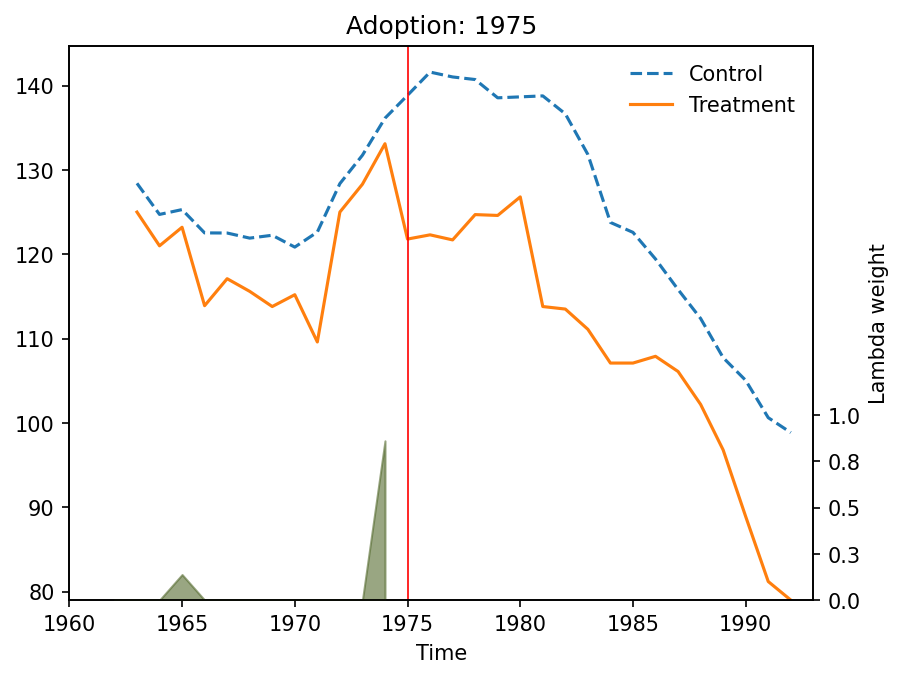
\includegraphics[width=\textwidth]{comparativa_figs/py_trends_1975.png}
  \caption{\py{} --- Cohorte 1975}
\end{subfigure}
\hfill
\begin{subfigure}[b]{0.48\textwidth}
  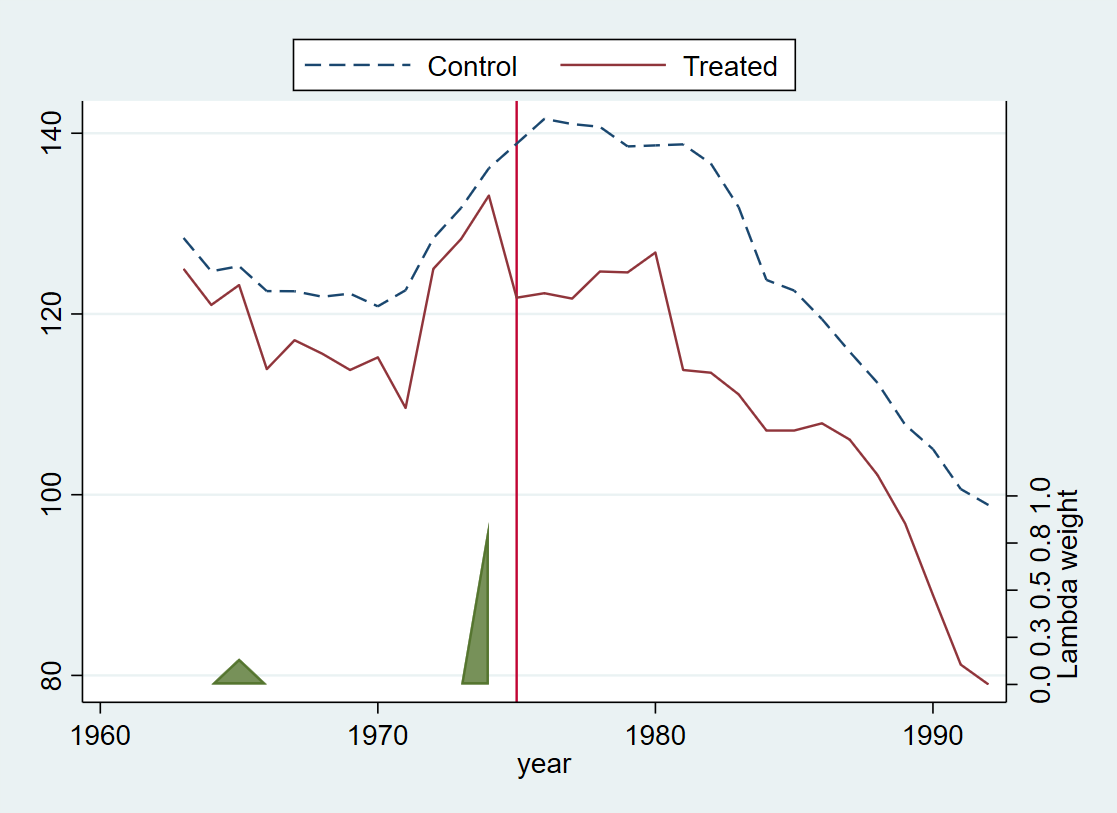
\includegraphics[width=\textwidth]{comparativa_figs/stata_trends_1975.png}
  \caption{\st{} --- Cohorte 1975}
\end{subfigure}
\caption{Trayectorias tratados vs control sint\'etico --- Adopci\'on 1975 (ATT$_\text{py}=-13.56$, ATT$_\text{st}\approx-13.56$)}
\end{figure}

% ------ Cohorte 1976 ------
\begin{figure}[H]
\centering
\begin{subfigure}[b]{0.48\textwidth}
  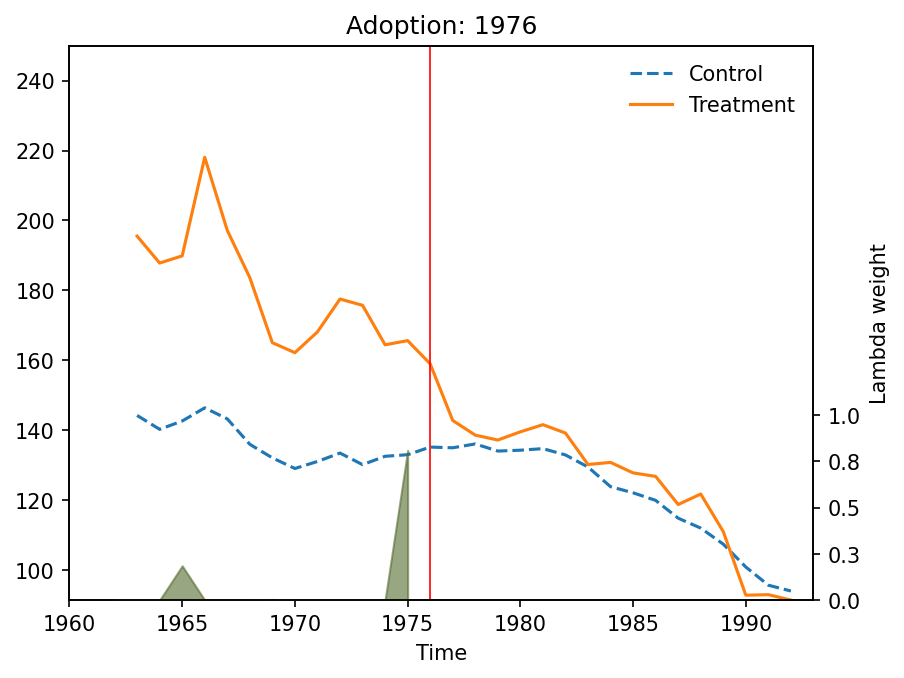
\includegraphics[width=\textwidth]{comparativa_figs/py_trends_1976.png}
  \caption{\py{} --- Cohorte 1976}
\end{subfigure}
\hfill
\begin{subfigure}[b]{0.48\textwidth}
  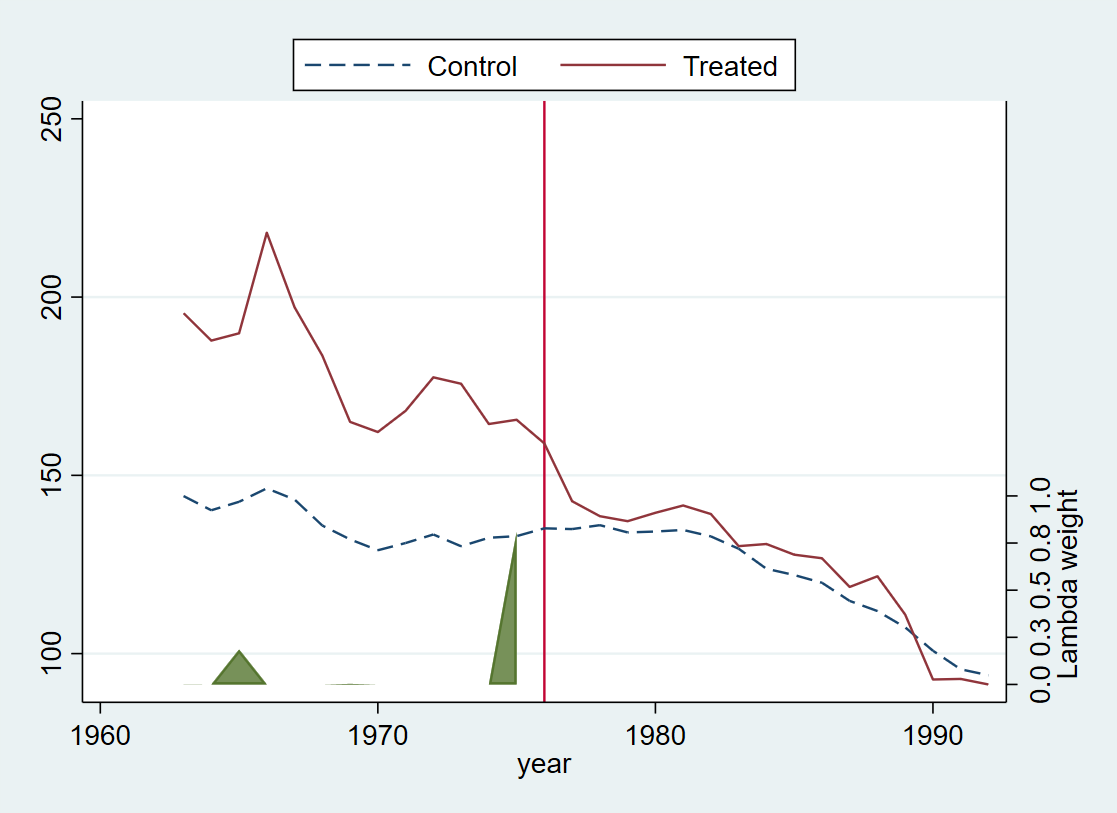
\includegraphics[width=\textwidth]{comparativa_figs/stata_trends_1976.png}
  \caption{\st{} --- Cohorte 1976}
\end{subfigure}
\caption{Trayectorias --- Adopci\'on 1976 (ATT$_\text{py}=-30.68$, mayor efecto por 2 estados tratados)}
\end{figure}

% ------ Cohorte 1978 ------
\begin{figure}[H]
\centering
\begin{subfigure}[b]{0.48\textwidth}
  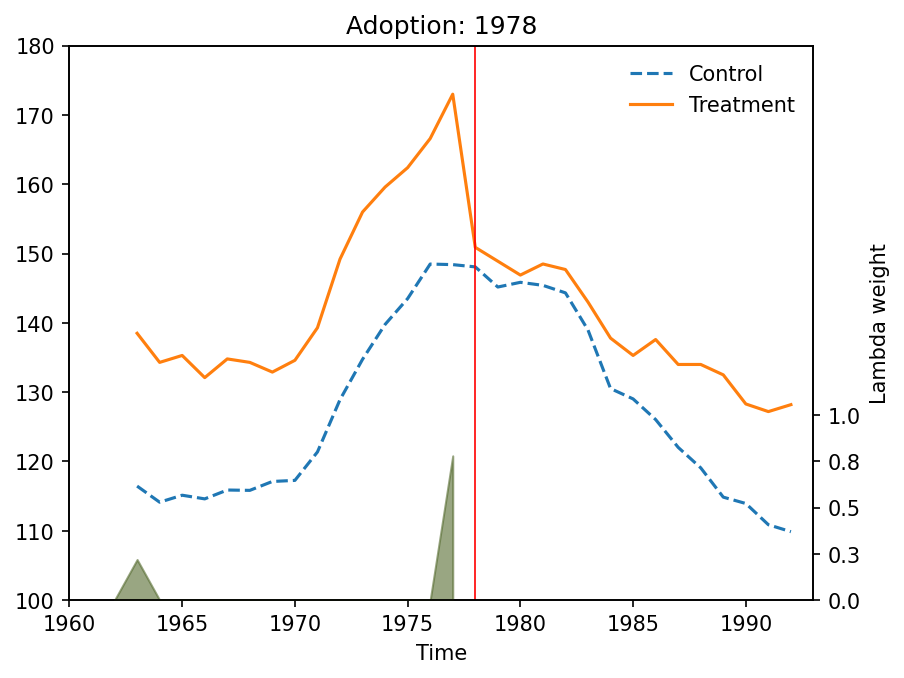
\includegraphics[width=\textwidth]{comparativa_figs/py_trends_1978.png}
  \caption{\py{} --- Cohorte 1978}
\end{subfigure}
\hfill
\begin{subfigure}[b]{0.48\textwidth}
  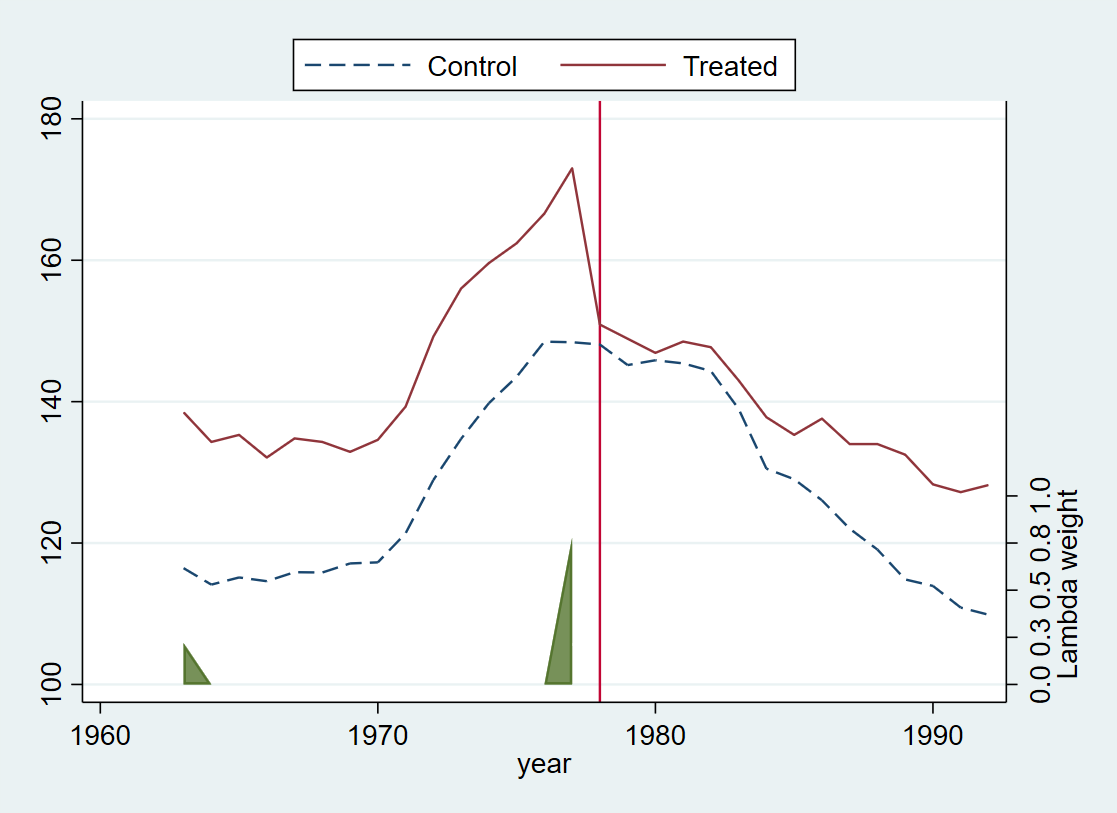
\includegraphics[width=\textwidth]{comparativa_figs/stata_trends_1978.png}
  \caption{\st{} --- Cohorte 1978}
\end{subfigure}
\caption{Trayectorias --- Adopci\'on 1978 (ATT$_\text{py}=-14.92$)}
\end{figure}

% ------ Cohorte 1979 ------
\begin{figure}[H]
\centering
\begin{subfigure}[b]{0.48\textwidth}
  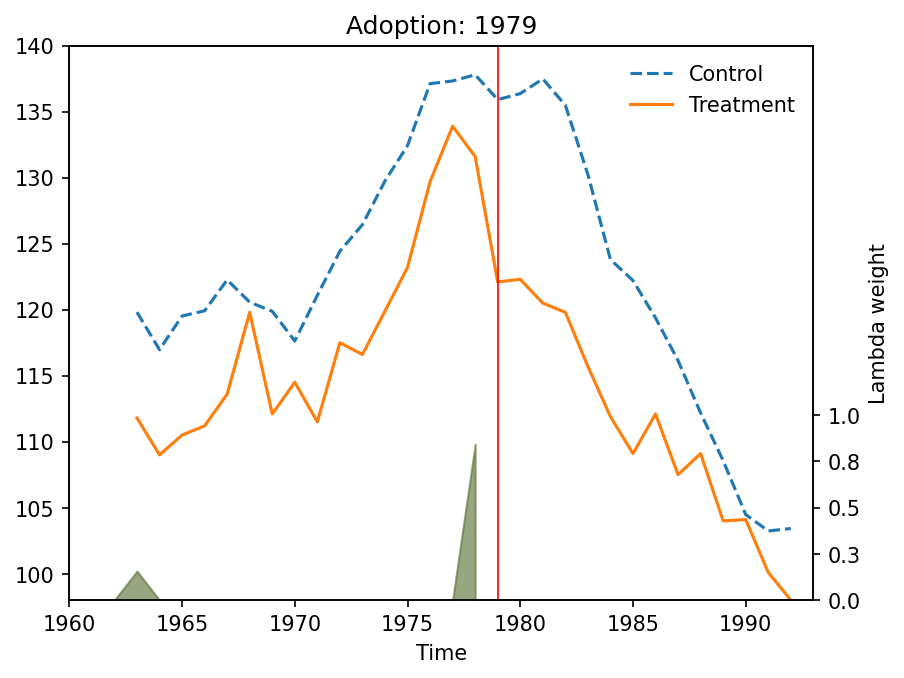
\includegraphics[width=\textwidth]{comparativa_figs/py_trends_1979.png}
  \caption{\py{} --- Cohorte 1979}
\end{subfigure}
\hfill
\begin{subfigure}[b]{0.48\textwidth}
  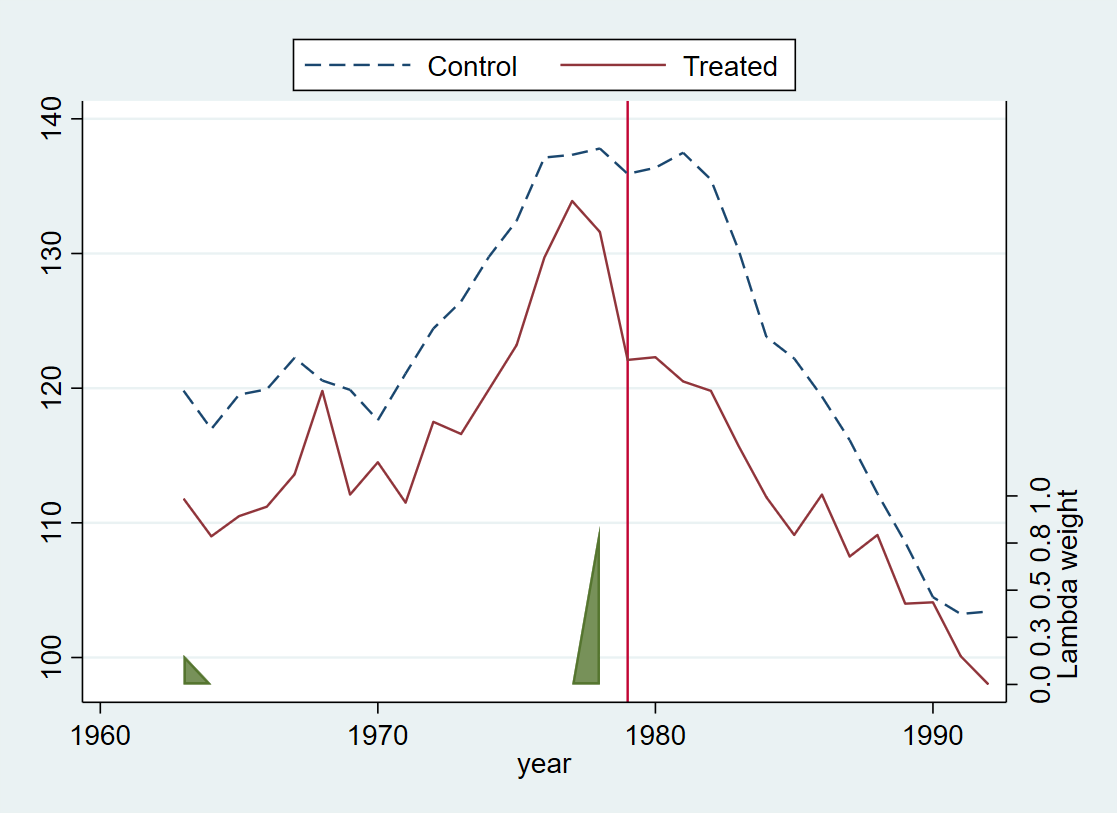
\includegraphics[width=\textwidth]{comparativa_figs/stata_trends_1979.png}
  \caption{\st{} --- Cohorte 1979}
\end{subfigure}
\caption{Trayectorias --- Adopci\'on 1979 (ATT$_\text{py}=-2.99$, efecto pequeño)}
\end{figure}

% ------ Cohorte 1981 ------
\begin{figure}[H]
\centering
\begin{subfigure}[b]{0.48\textwidth}
  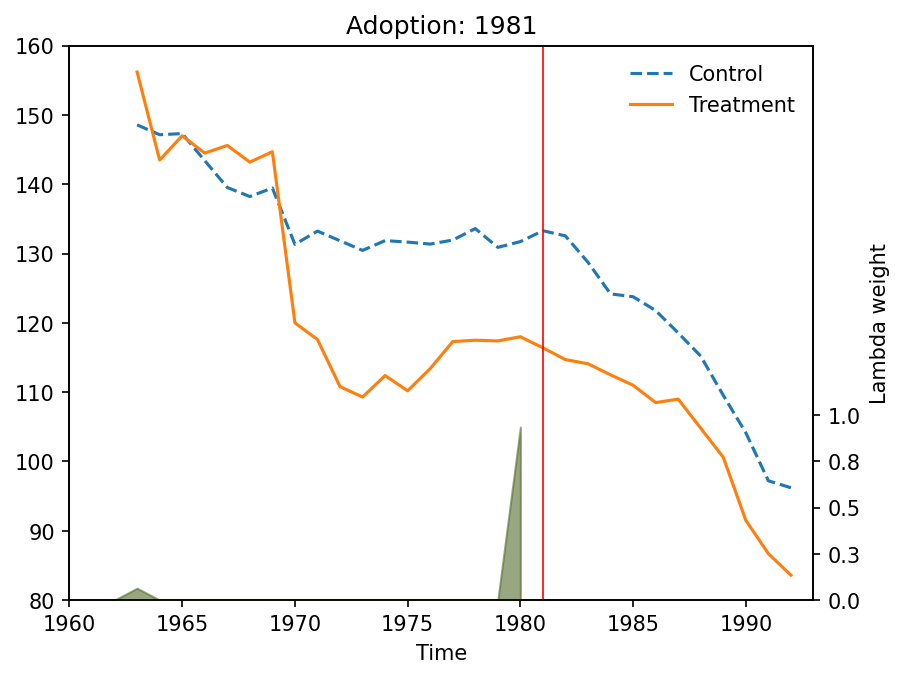
\includegraphics[width=\textwidth]{comparativa_figs/py_trends_1981.png}
  \caption{\py{} --- Cohorte 1981}
\end{subfigure}
\hfill
\begin{subfigure}[b]{0.48\textwidth}
  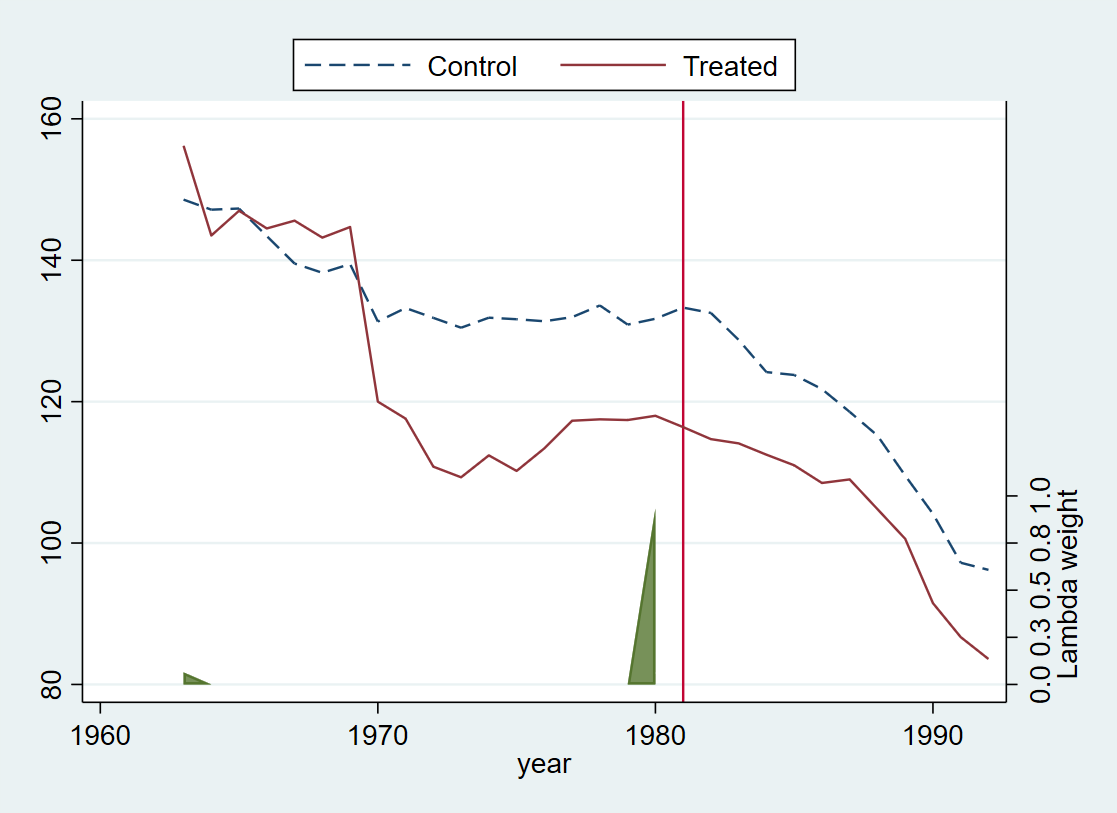
\includegraphics[width=\textwidth]{comparativa_figs/stata_trends_1981.png}
  \caption{\st{} --- Cohorte 1981}
\end{subfigure}
\caption{Trayectorias --- Adopci\'on 1981 (ATT$_\text{py}=-0.29$, efecto pr\'acticamente nulo)}
\end{figure}

% ------ Cohorte 1983 ------
\begin{figure}[H]
\centering
\begin{subfigure}[b]{0.48\textwidth}
  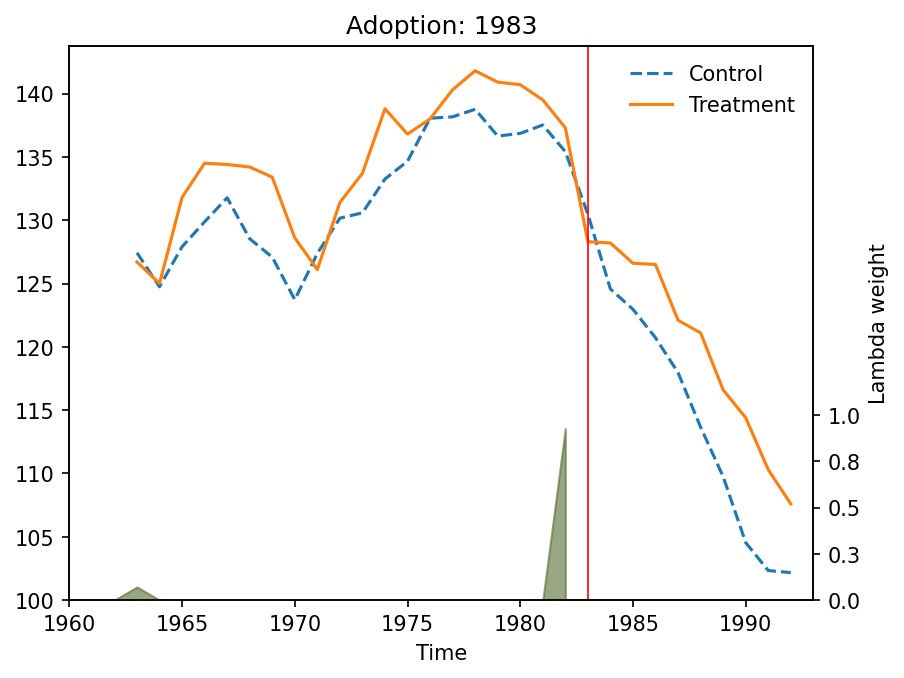
\includegraphics[width=\textwidth]{comparativa_figs/py_trends_1983.png}
  \caption{\py{} --- Cohorte 1983}
\end{subfigure}
\hfill
\begin{subfigure}[b]{0.48\textwidth}
  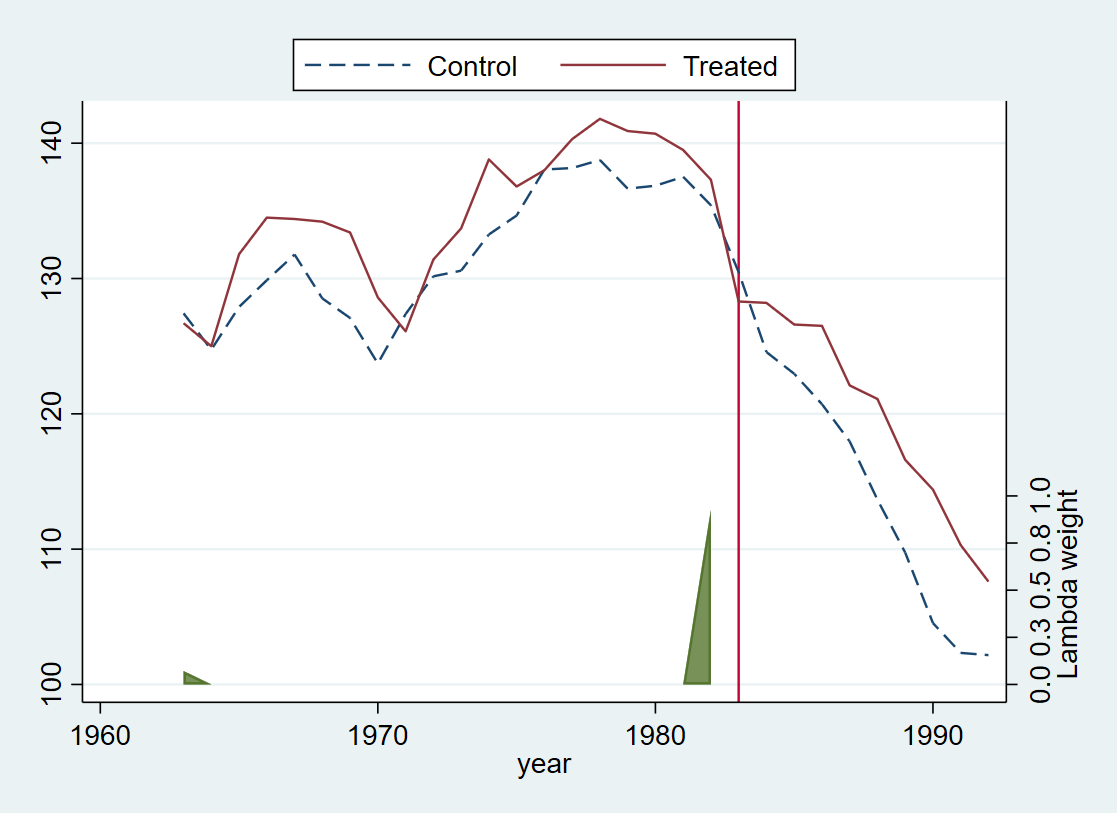
\includegraphics[width=\textwidth]{comparativa_figs/stata_trends_1983.png}
  \caption{\st{} --- Cohorte 1983}
\end{subfigure}
\caption{Trayectorias --- Adopci\'on 1983 (ATT$_\text{py}=+3.56$, efecto positivo)}
\end{figure}

% ------ Cohorte 1986 ------
\begin{figure}[H]
\centering
\begin{subfigure}[b]{0.48\textwidth}
  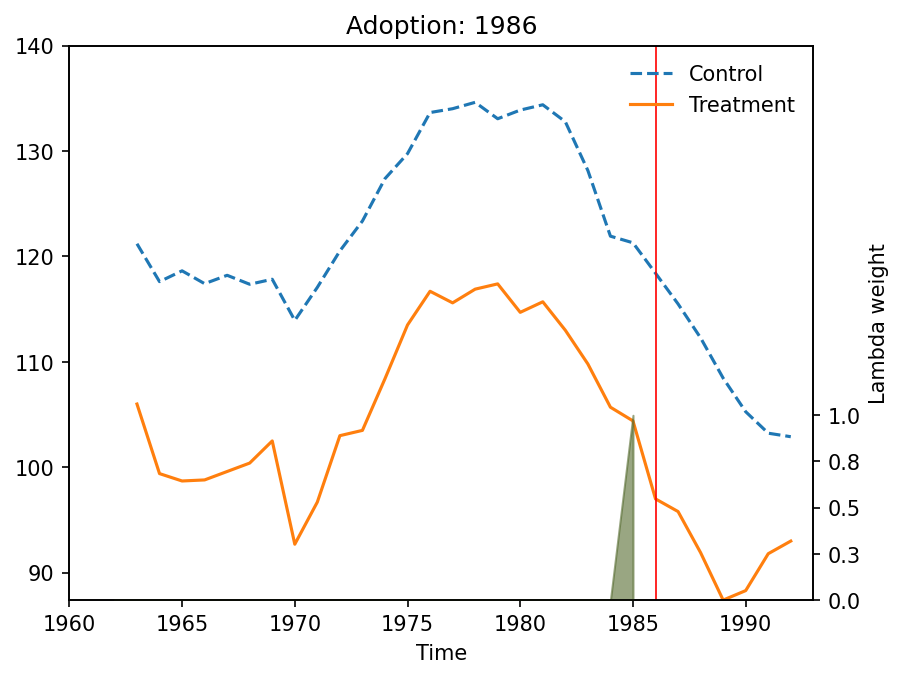
\includegraphics[width=\textwidth]{comparativa_figs/py_trends_1986.png}
  \caption{\py{} --- Cohorte 1986}
\end{subfigure}
\hfill
\begin{subfigure}[b]{0.48\textwidth}
  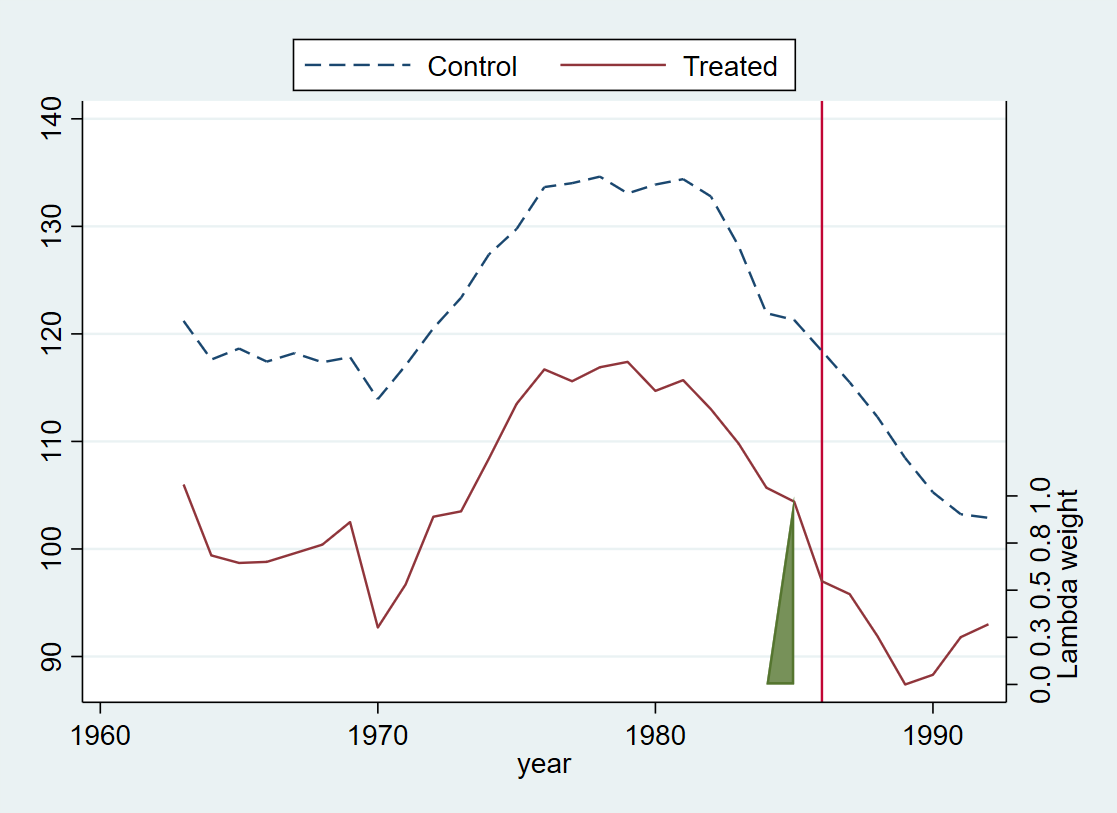
\includegraphics[width=\textwidth]{comparativa_figs/stata_trends_1986.png}
  \caption{\st{} --- Cohorte 1986}
\end{subfigure}
\caption{Trayectorias --- Adopci\'on 1986 (ATT$_\text{py}=-0.37$, pocos periodos post)}
\end{figure}

% ============================================================
\newpage
\section{Experimento 6: Gráficos de Pesos de Unidades de Control ($\hat\omega$)}
% ============================================================

Los pesos $\hat\omega$ miden la contribuci\'on de cada unidad de control al contrafactual sint\'etico. Un peso alto indica que esa unidad de control es ``similar'' a los tratados en el pre-período. En \py{} (izquierda), el eje Y muestra la diferencia $\hat\omega_i (Y_i \hat\lambda_\text{post} - Y_i \hat\lambda_\text{pre})$, es decir, el ajuste post-pre ponderado. En \st{} (derecha), el eje Y muestra el peso $\hat\omega_i$ directamente, con el tamaño del punto proporcional al peso.

% ------ Cohorte 1975 ------
\begin{figure}[H]
\centering
\begin{subfigure}[b]{0.48\textwidth}
  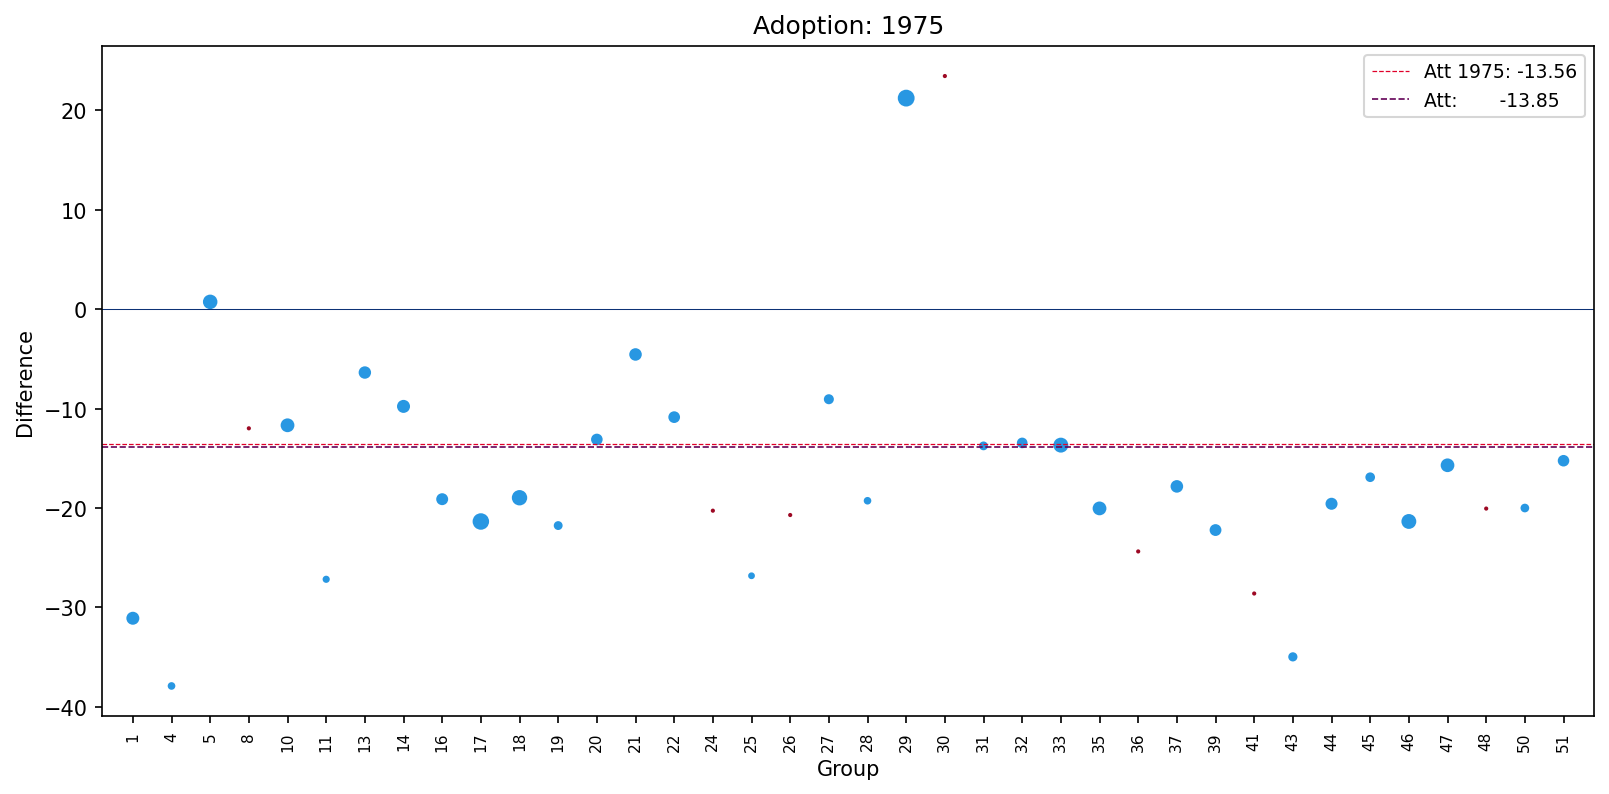
\includegraphics[width=\textwidth]{comparativa_figs/py_weights_1975.png}
  \caption{\py{} --- Pesos $\hat\omega$, Cohorte 1975}
\end{subfigure}
\hfill
\begin{subfigure}[b]{0.48\textwidth}
  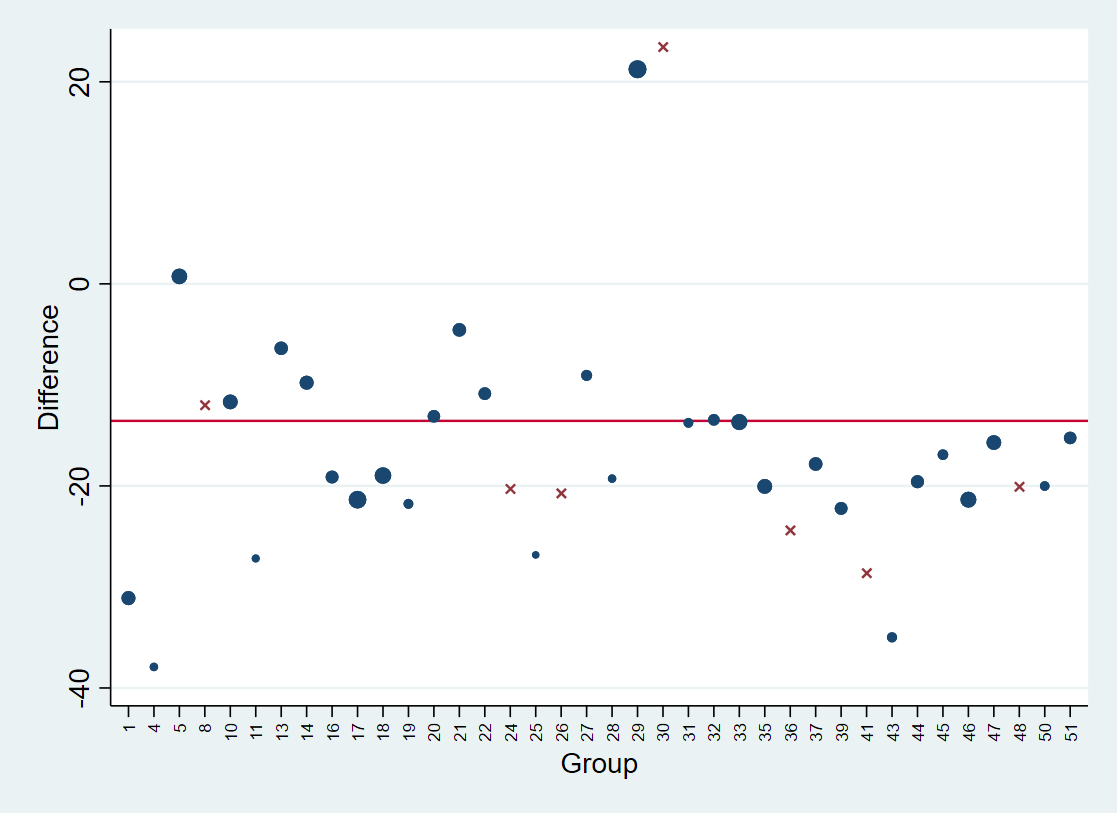
\includegraphics[width=\textwidth]{comparativa_figs/stata_weights_1975.png}
  \caption{\st{} --- Pesos $\hat\omega$, Cohorte 1975}
\end{subfigure}
\caption{Pesos de unidades de control --- Adopci\'on 1975}
\end{figure}

% ------ Cohorte 1976 ------
\begin{figure}[H]
\centering
\begin{subfigure}[b]{0.48\textwidth}
  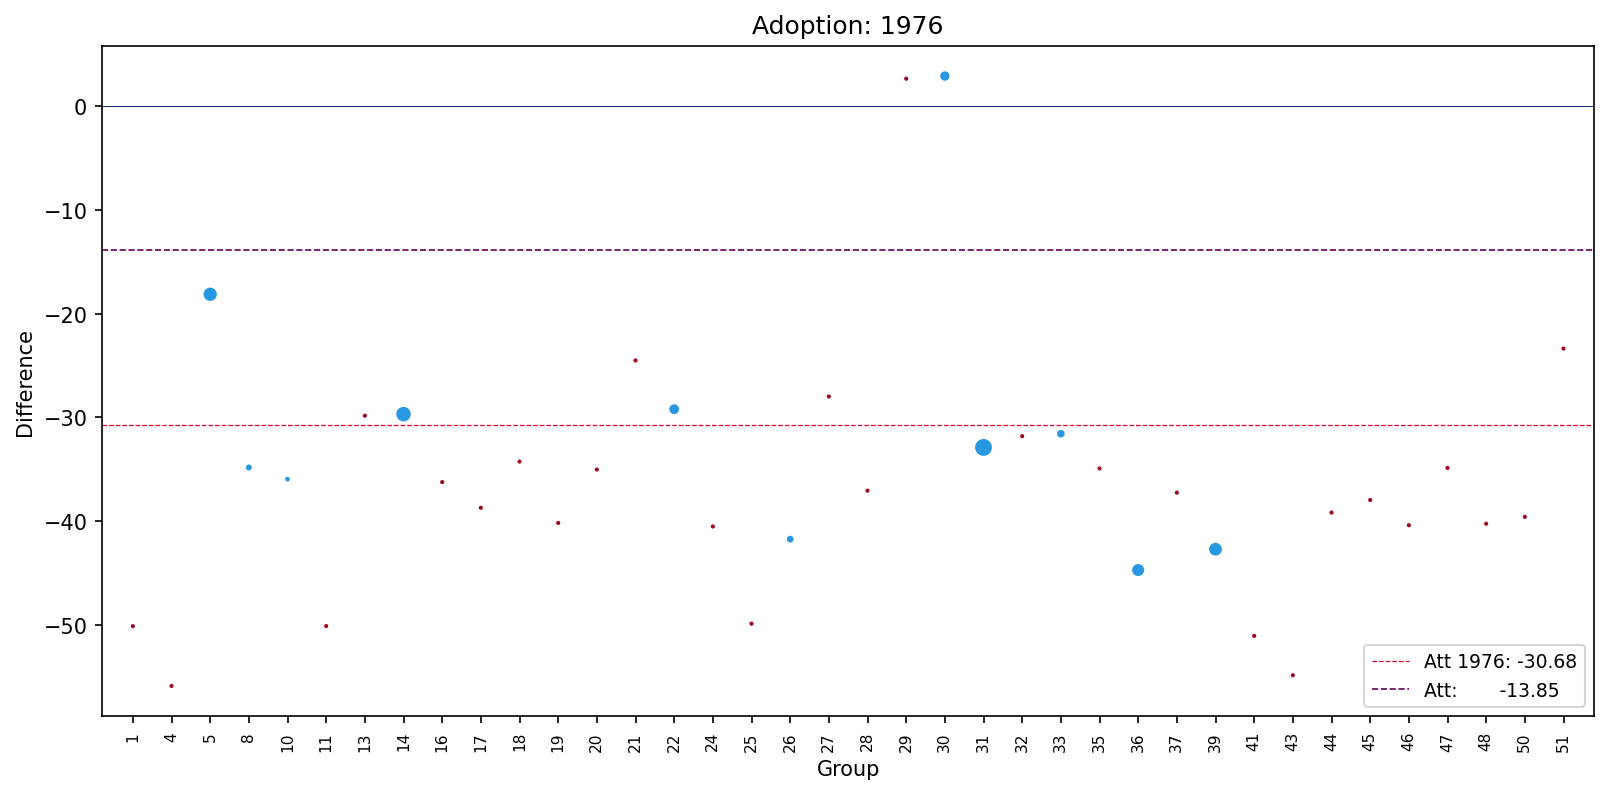
\includegraphics[width=\textwidth]{comparativa_figs/py_weights_1976.png}
  \caption{\py{} --- Pesos $\hat\omega$, Cohorte 1976}
\end{subfigure}
\hfill
\begin{subfigure}[b]{0.48\textwidth}
  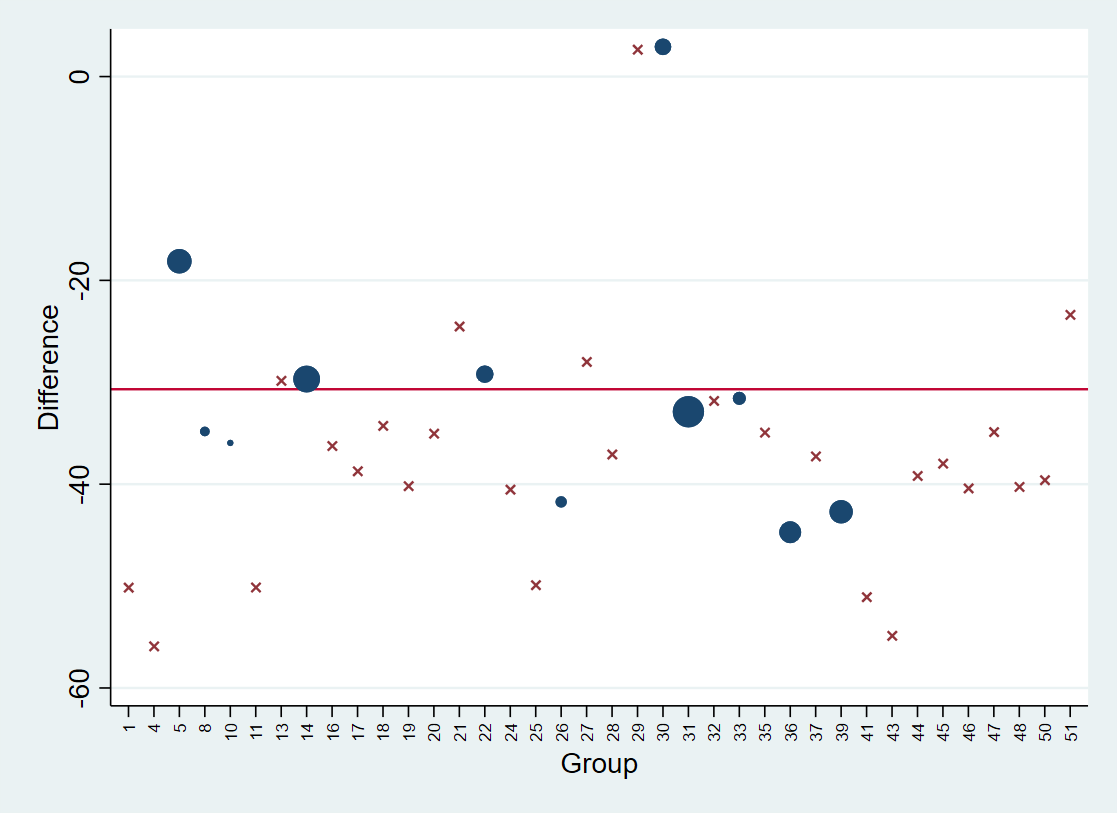
\includegraphics[width=\textwidth]{comparativa_figs/stata_weights_1976.png}
  \caption{\st{} --- Pesos $\hat\omega$, Cohorte 1976}
\end{subfigure}
\caption{Pesos de unidades de control --- Adopci\'on 1976}
\end{figure}

% ------ Cohorte 1978 ------
\begin{figure}[H]
\centering
\begin{subfigure}[b]{0.48\textwidth}
  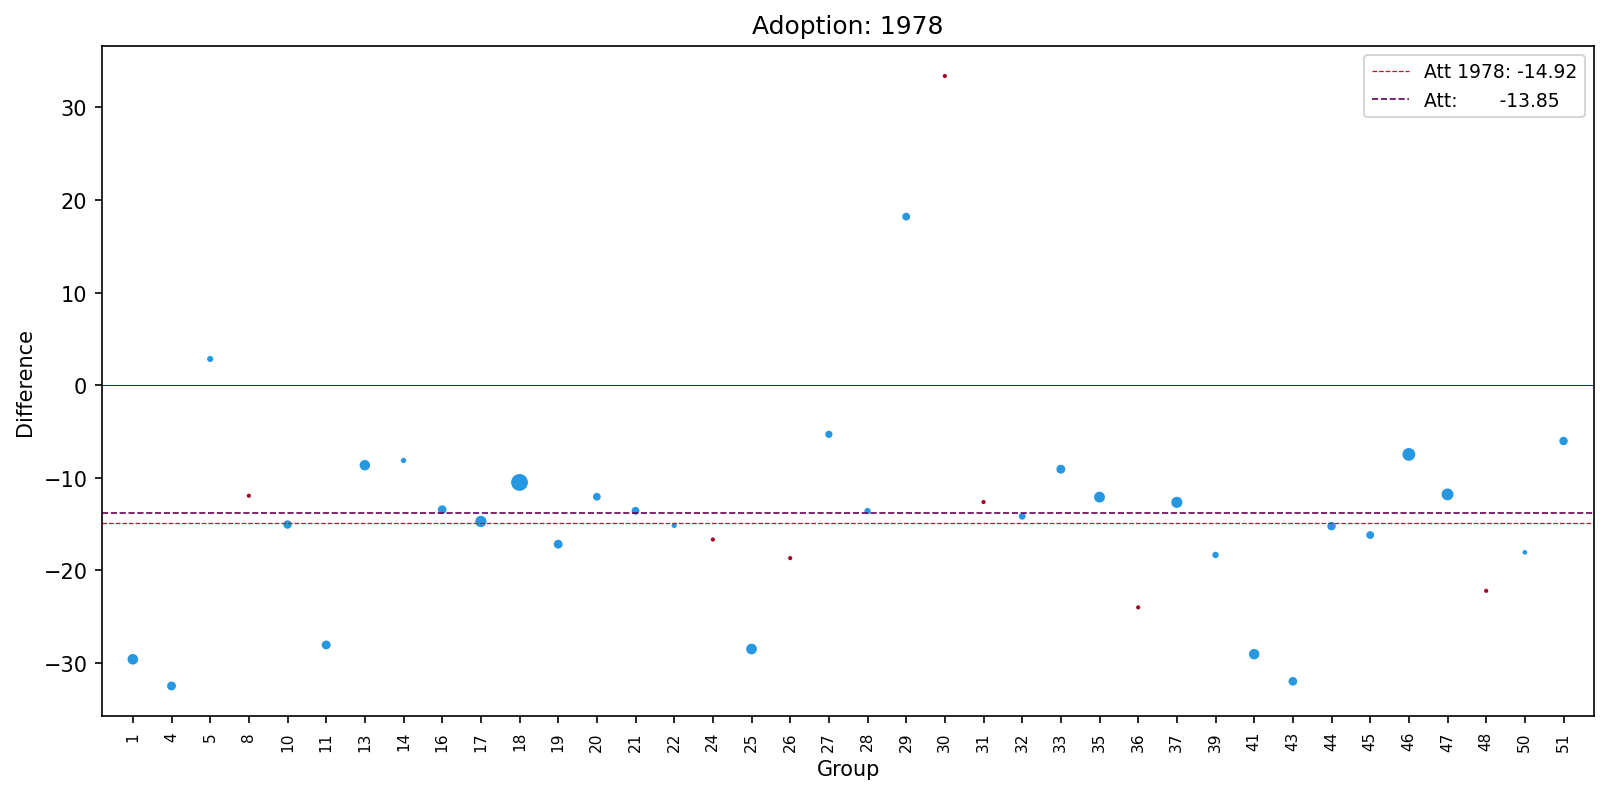
\includegraphics[width=\textwidth]{comparativa_figs/py_weights_1978.png}
  \caption{\py{} --- Pesos $\hat\omega$, Cohorte 1978}
\end{subfigure}
\hfill
\begin{subfigure}[b]{0.48\textwidth}
  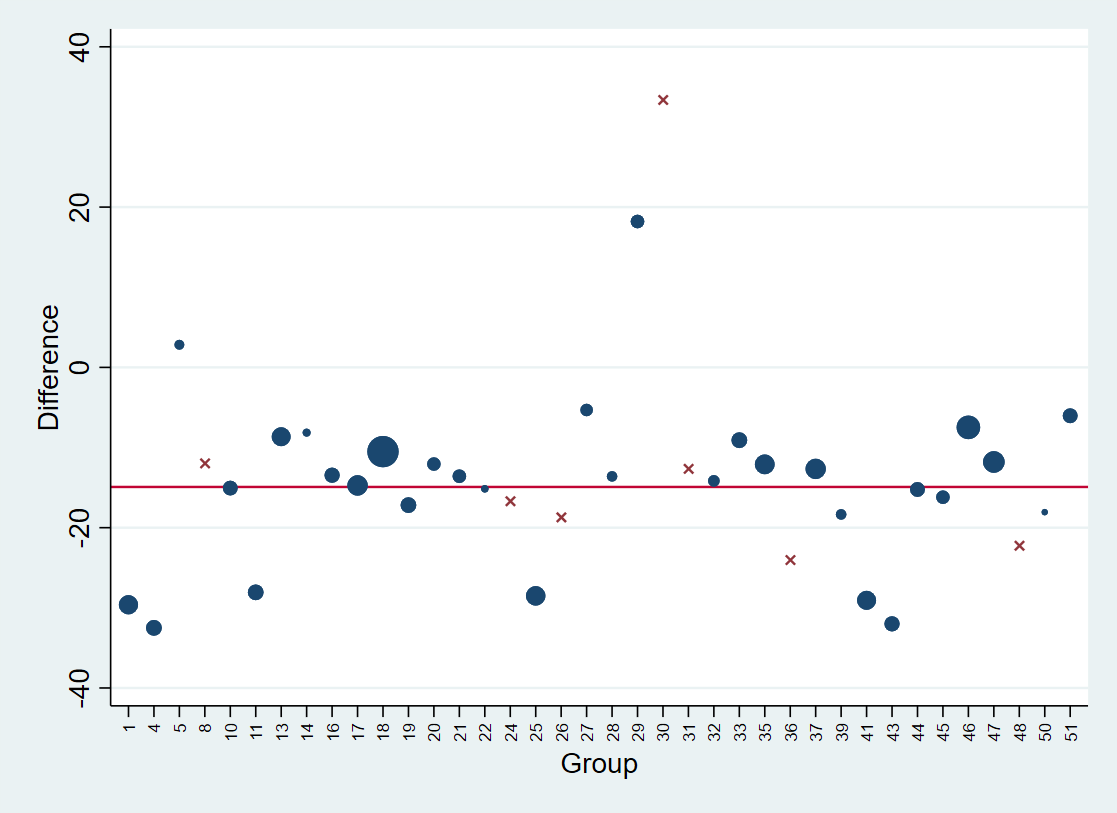
\includegraphics[width=\textwidth]{comparativa_figs/stata_weights_1978.png}
  \caption{\st{} --- Pesos $\hat\omega$, Cohorte 1978}
\end{subfigure}
\caption{Pesos de unidades de control --- Adopci\'on 1978}
\end{figure}

% ------ Cohorte 1979 ------
\begin{figure}[H]
\centering
\begin{subfigure}[b]{0.48\textwidth}
  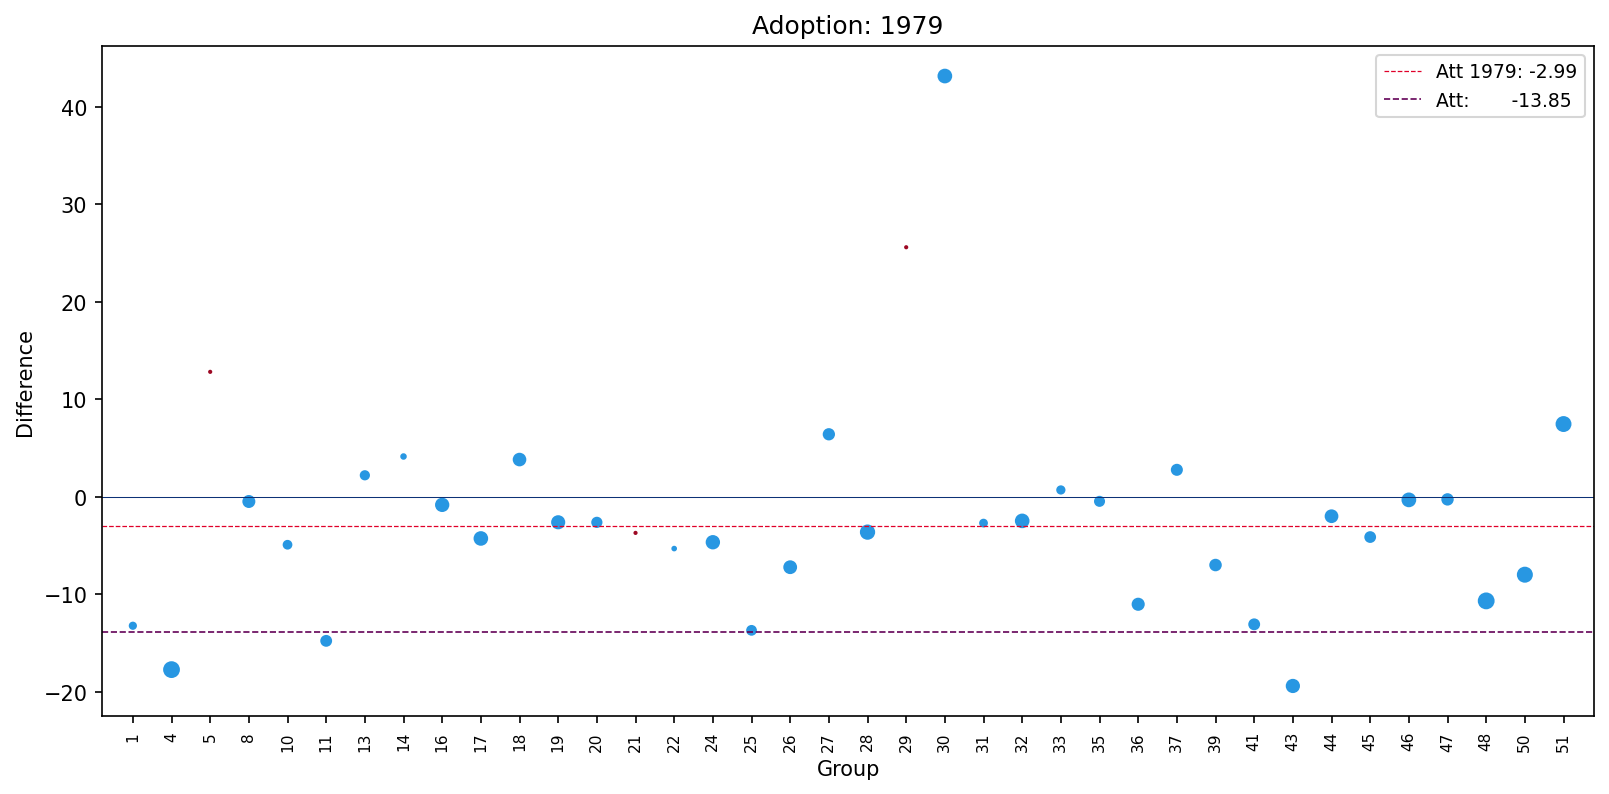
\includegraphics[width=\textwidth]{comparativa_figs/py_weights_1979.png}
  \caption{\py{} --- Pesos $\hat\omega$, Cohorte 1979}
\end{subfigure}
\hfill
\begin{subfigure}[b]{0.48\textwidth}
  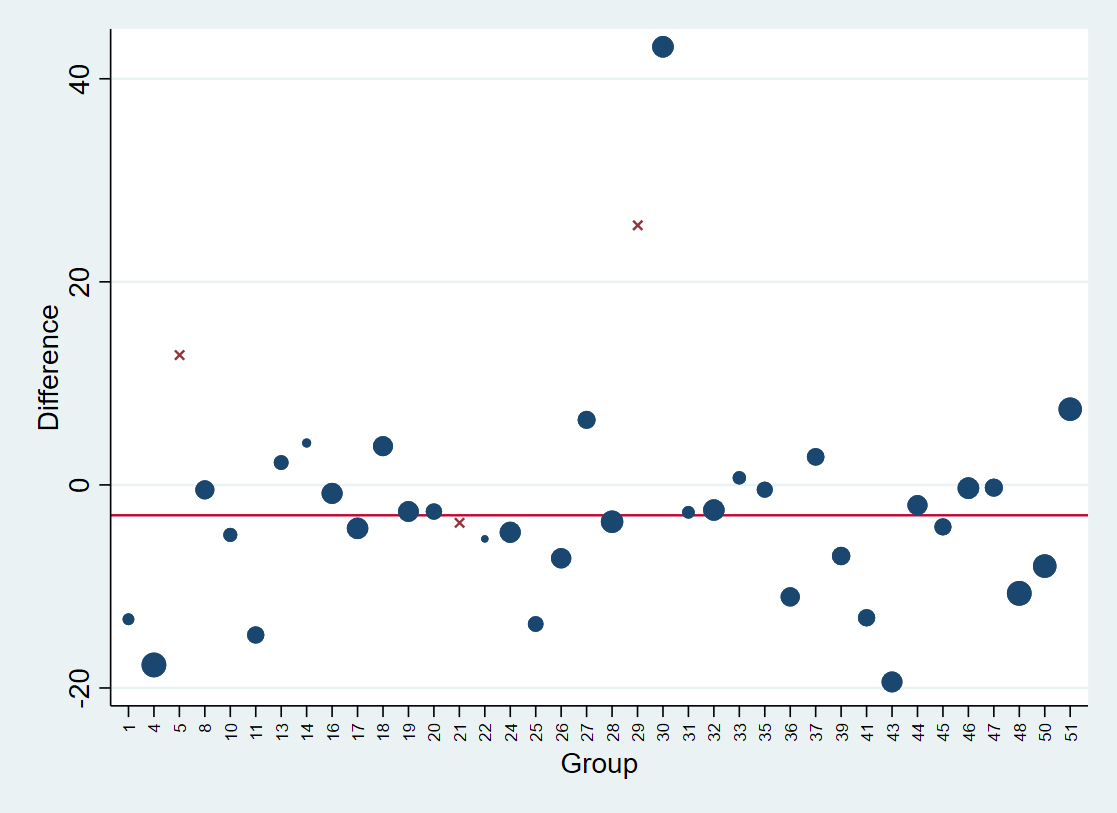
\includegraphics[width=\textwidth]{comparativa_figs/stata_weights_1979.png}
  \caption{\st{} --- Pesos $\hat\omega$, Cohorte 1979}
\end{subfigure}
\caption{Pesos de unidades de control --- Adopci\'on 1979}
\end{figure}

% ------ Cohorte 1981 ------
\begin{figure}[H]
\centering
\begin{subfigure}[b]{0.48\textwidth}
  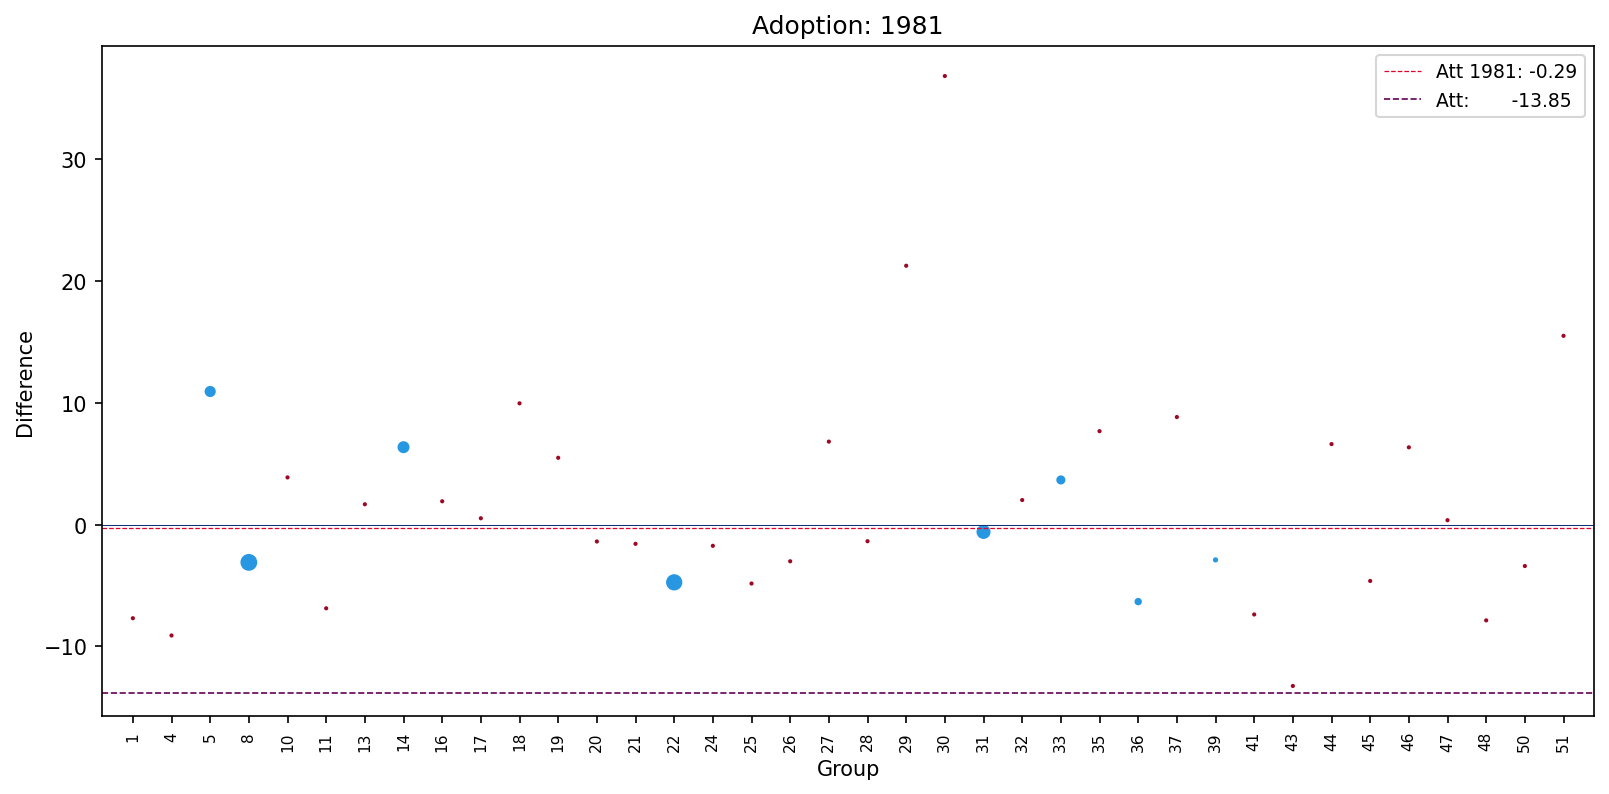
\includegraphics[width=\textwidth]{comparativa_figs/py_weights_1981.png}
  \caption{\py{} --- Pesos $\hat\omega$, Cohorte 1981}
\end{subfigure}
\hfill
\begin{subfigure}[b]{0.48\textwidth}
  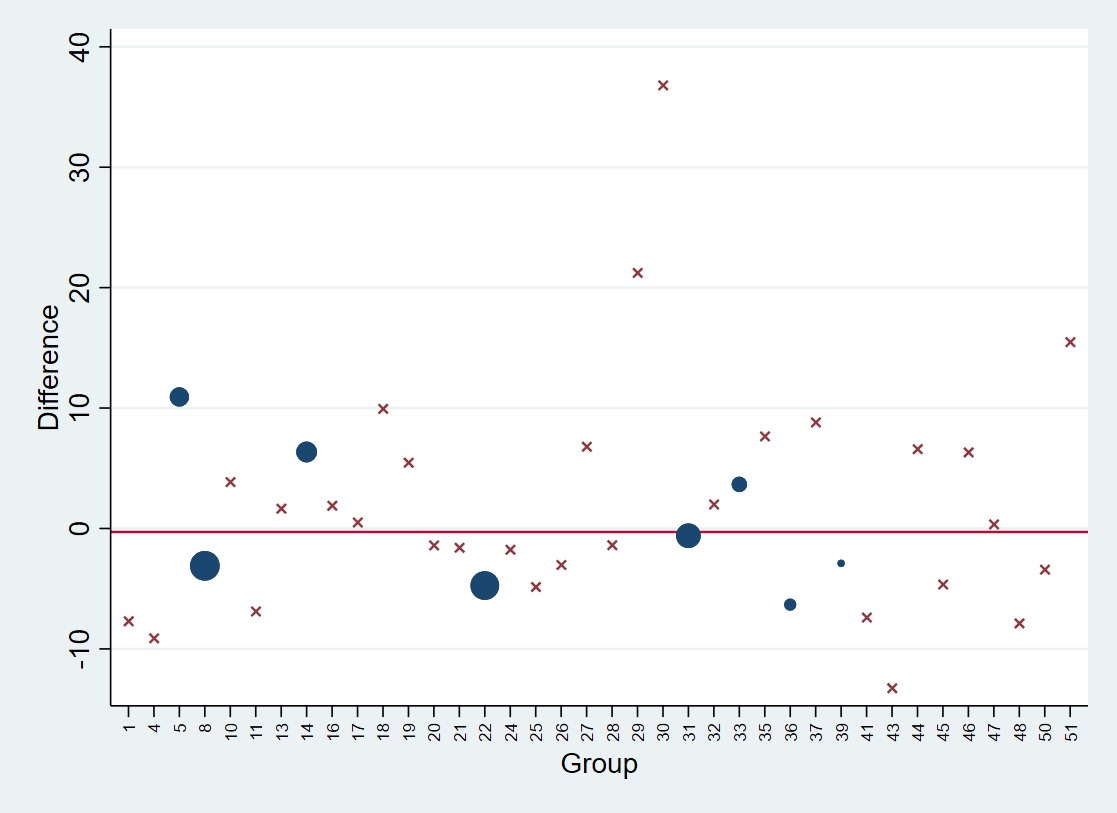
\includegraphics[width=\textwidth]{comparativa_figs/stata_weights_1981.png}
  \caption{\st{} --- Pesos $\hat\omega$, Cohorte 1981}
\end{subfigure}
\caption{Pesos de unidades de control --- Adopci\'on 1981}
\end{figure}

% ------ Cohorte 1983 ------
\begin{figure}[H]
\centering
\begin{subfigure}[b]{0.48\textwidth}
  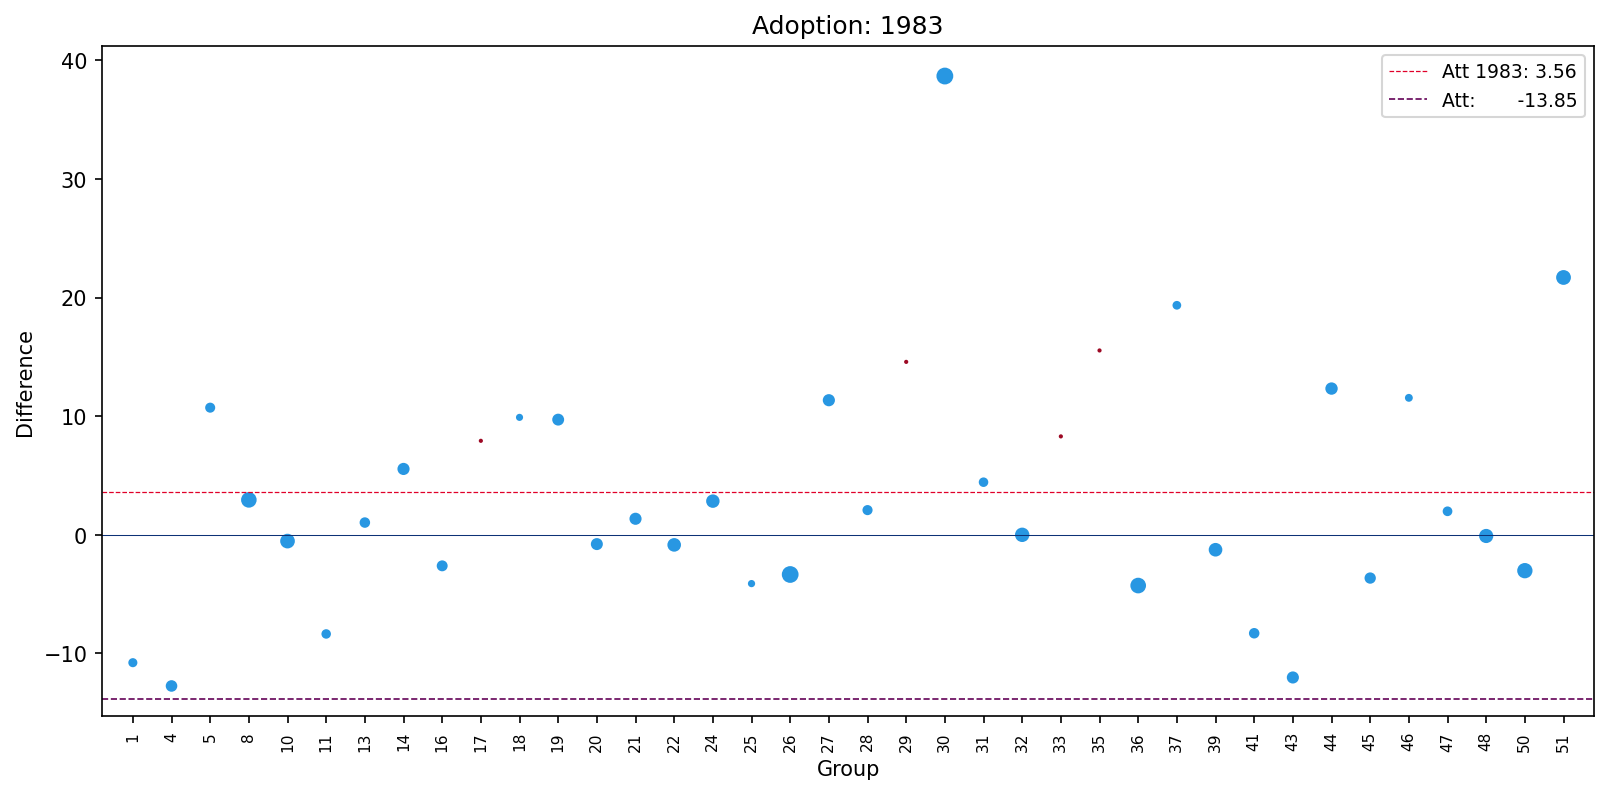
\includegraphics[width=\textwidth]{comparativa_figs/py_weights_1983.png}
  \caption{\py{} --- Pesos $\hat\omega$, Cohorte 1983}
\end{subfigure}
\hfill
\begin{subfigure}[b]{0.48\textwidth}
  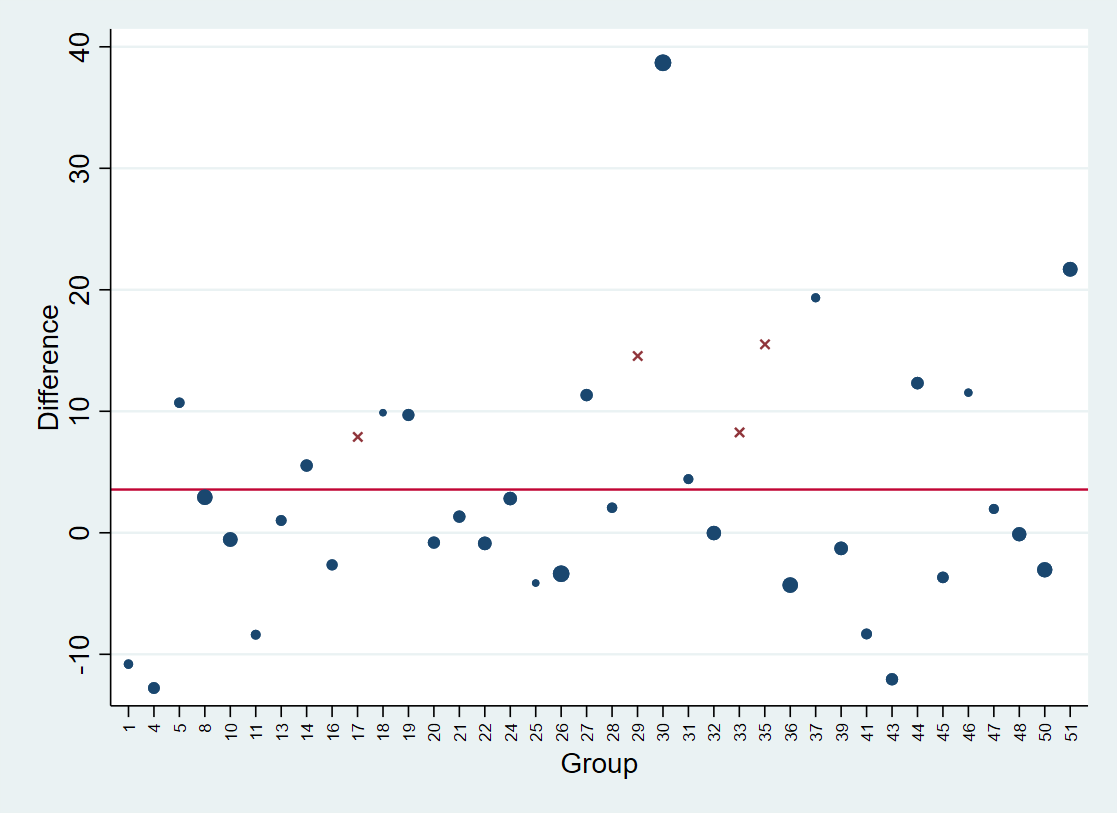
\includegraphics[width=\textwidth]{comparativa_figs/stata_weights_1983.png}
  \caption{\st{} --- Pesos $\hat\omega$, Cohorte 1983}
\end{subfigure}
\caption{Pesos de unidades de control --- Adopci\'on 1983}
\end{figure}

% ------ Cohorte 1986 ------
\begin{figure}[H]
\centering
\begin{subfigure}[b]{0.48\textwidth}
  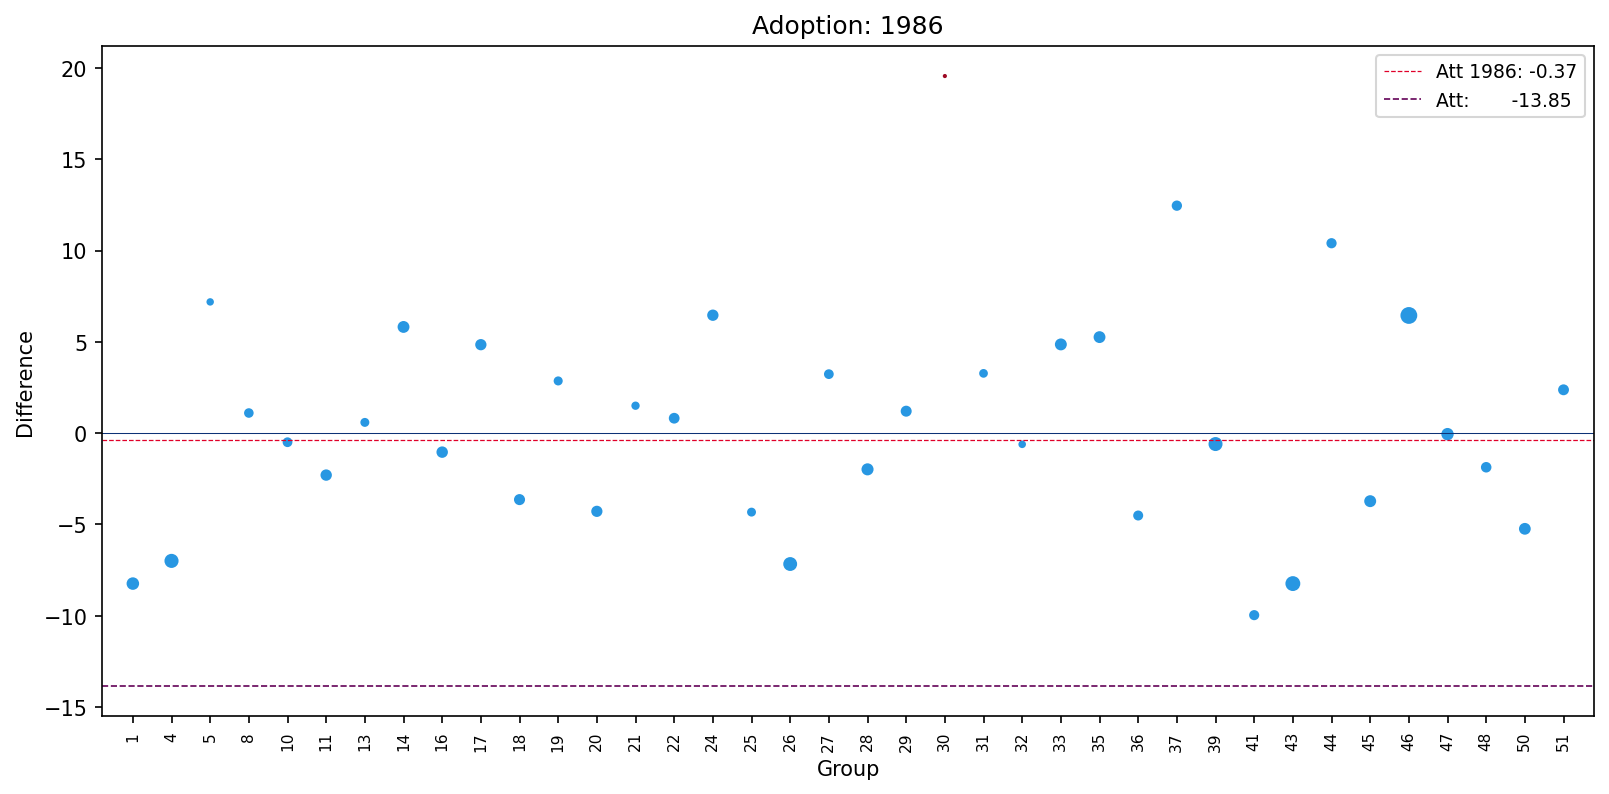
\includegraphics[width=\textwidth]{comparativa_figs/py_weights_1986.png}
  \caption{\py{} --- Pesos $\hat\omega$, Cohorte 1986}
\end{subfigure}
\hfill
\begin{subfigure}[b]{0.48\textwidth}
  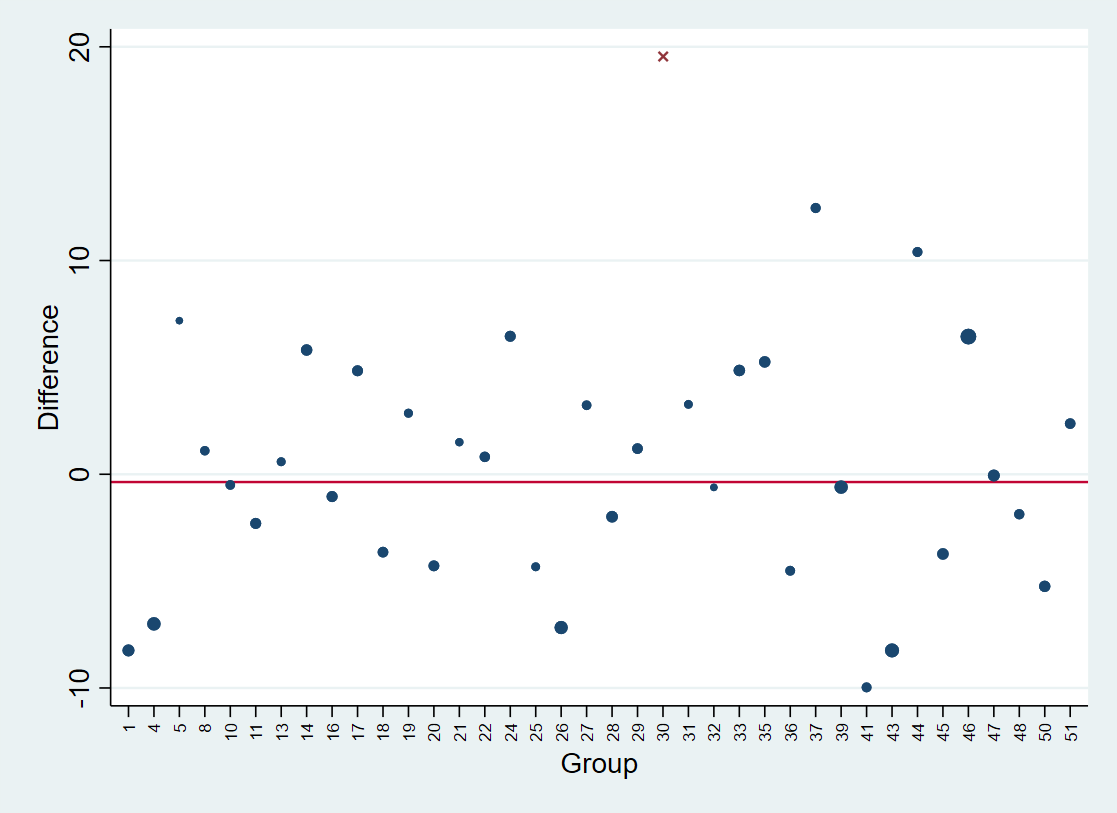
\includegraphics[width=\textwidth]{comparativa_figs/stata_weights_1986.png}
  \caption{\st{} --- Pesos $\hat\omega$, Cohorte 1986}
\end{subfigure}
\caption{Pesos de unidades de control --- Adopci\'on 1986}
\end{figure}

% ============================================================
\newpage
\section{Experimento 7: Comparaci\'on de Pesos ($\hat{\omega}$ y $\hat{\lambda}$)}
% ============================================================

\subsection*{Resumen de diferencias}

\begin{table}[H]
\centering
\caption{Diferencia m\'axima absoluta entre pesos Python y Stata}
\label{tab:weight_summary}
\begin{tabular}{lcc}
\toprule
M\'etodo & $\max|\hat{\omega}^{\text{Py}} - \hat{\omega}^{\text{Stata}}|$ &
           $\max|\hat{\lambda}^{\text{Py}} - \hat{\lambda}^{\text{Stata}}|$ \\
\midrule
SDID & $4{.}8 \times 10^{-8}$ & $4{.}0 \times 10^{-8}$ \\
SC   & $5{.}0 \times 10^{-8}$ & $0$ (exacto) \\
DiD  & $1{.}1 \times 10^{-8}$ & $4{.}4 \times 10^{-8}$ \\
\bottomrule
\end{tabular}\\[0.4em]
{\small Las diferencias son acumulaciones de redondeo del algoritmo Frank-Wolfe en distintas implementaciones
(Mata/Stata vs NumPy/Python). Ambos paquetes usan el \textbf{mismo criterio de convergencia}
$(10^{-5}\cdot\hat\sigma_t)^2$ y el mismo n\'umero m\'aximo de iteraciones (10\,000).
Los pesos coinciden a \textbf{8 d\'ecimales} en todos los m\'etodos y cohortes; a 4 decimales son \textbf{id\'enticos}.}
\end{table}

\subsection*{Pesos temporales $\hat{\lambda}$ por m\'etodo y cohorte}

Las tablas siguientes muestran $\hat{\lambda}_t$ para cada a\~no pre-tratamiento
y cohorte (solo filas con $\hat{\lambda}_t > 10^{-8}$; los a\~nos no mostrados tienen $\hat{\lambda}_t = 0$).
Los valores entre Python y Stata son id\'enticos a 4 decimales.

\begin{table}[H]
\centering
\caption{Pesos temporales ($\hat{\lambda}$) --- SDID. Python $=$ Stata a 4 decimales.}
\label{tab:lambda_sdid}
\small
\begin{tabular}{rrrrrrrr}
\toprule
A\~{n}o & 1975 & 1976 & 1978 & 1979 & 1981 & 1983 & 1986 \\
\midrule
1963 & 0 & 0.0011 & 0.2195 & 0.1566 & 0.0641 & 0.0711 & 0 \\
1965 & 0.1382 & 0.1854 & 0 & 0 & 0 & 0 & 0 \\
1969 & 0 & 0.0034 & 0 & 0 & 0 & 0 & 0 \\
1974 & 0.8618 & 0 & 0 & 0 & 0 & 0 & 0 \\
1975 & -- & 0.8100 & 0 & 0 & 0 & 0 & 0 \\
1977 & -- & -- & 0.7805 & 0 & 0 & 0 & 0 \\
1978 & -- & -- & -- & 0.8434 & 0 & 0 & 0 \\
1980 & -- & -- & -- & -- & 0.9359 & 0 & 0 \\
1982 & -- & -- & -- & -- & -- & 0.9289 & 0 \\
1985 & -- & -- & -- & -- & -- & -- & 1.0000 \\
\bottomrule
\end{tabular}
\end{table}

\begin{table}[H]
\centering
\caption{Pesos temporales ($\hat{\lambda}$) --- SC. Python $=$ Stata a 4 decimales.}
\label{tab:lambda_sc}
\small
\begin{tabular}{rrrrrrrr}
\toprule
A\~{n}o & 1975 & 1976 & 1978 & 1979 & 1981 & 1983 & 1986 \\
\midrule
\multicolumn{8}{c}{\textit{SC: $\hat{\lambda}_t = 0\ \forall\,t$ (sin ponderaci\'on temporal pre-per\'iodo).}} \\
\bottomrule
\end{tabular}
\end{table}

\begin{table}[H]
\centering
\caption{Pesos temporales ($\hat{\lambda}$) --- DiD. Python $=$ Stata a 4 decimales.}
\label{tab:lambda_did}
\small
\begin{tabular}{rrrrrrrr}
\toprule
A\~{n}o & 1975 & 1976 & 1978 & 1979 & 1981 & 1983 & 1986 \\
\midrule
1963 & 0.0833 & 0.0769 & 0.0667 & 0.0625 & 0.0556 & 0.0500 & 0.0435 \\
1964 & 0.0833 & 0.0769 & 0.0667 & 0.0625 & 0.0556 & 0.0500 & 0.0435 \\
1965 & 0.0833 & 0.0769 & 0.0667 & 0.0625 & 0.0556 & 0.0500 & 0.0435 \\
1966 & 0.0833 & 0.0769 & 0.0667 & 0.0625 & 0.0556 & 0.0500 & 0.0435 \\
1967 & 0.0833 & 0.0769 & 0.0667 & 0.0625 & 0.0556 & 0.0500 & 0.0435 \\
1968 & 0.0833 & 0.0769 & 0.0667 & 0.0625 & 0.0556 & 0.0500 & 0.0435 \\
1969 & 0.0833 & 0.0769 & 0.0667 & 0.0625 & 0.0556 & 0.0500 & 0.0435 \\
1970 & 0.0833 & 0.0769 & 0.0667 & 0.0625 & 0.0556 & 0.0500 & 0.0435 \\
1971 & 0.0833 & 0.0769 & 0.0667 & 0.0625 & 0.0556 & 0.0500 & 0.0435 \\
1972 & 0.0833 & 0.0769 & 0.0667 & 0.0625 & 0.0556 & 0.0500 & 0.0435 \\
1973 & 0.0833 & 0.0769 & 0.0667 & 0.0625 & 0.0556 & 0.0500 & 0.0435 \\
1974 & 0.0833 & 0.0769 & 0.0667 & 0.0625 & 0.0556 & 0.0500 & 0.0435 \\
1975 & -- & 0.0769 & 0.0667 & 0.0625 & 0.0556 & 0.0500 & 0.0435 \\
1976 & -- & -- & 0.0667 & 0.0625 & 0.0556 & 0.0500 & 0.0435 \\
1977 & -- & -- & 0.0667 & 0.0625 & 0.0556 & 0.0500 & 0.0435 \\
1978 & -- & -- & -- & 0.0625 & 0.0556 & 0.0500 & 0.0435 \\
1979 & -- & -- & -- & -- & 0.0556 & 0.0500 & 0.0435 \\
1980 & -- & -- & -- & -- & 0.0556 & 0.0500 & 0.0435 \\
1981 & -- & -- & -- & -- & -- & 0.0500 & 0.0435 \\
1982 & -- & -- & -- & -- & -- & 0.0500 & 0.0435 \\
1983 & -- & -- & -- & -- & -- & -- & 0.0435 \\
1984 & -- & -- & -- & -- & -- & -- & 0.0435 \\
1985 & -- & -- & -- & -- & -- & -- & 0.0435 \\
\bottomrule
\end{tabular}
\end{table}

\subsection*{Pesos de unidades de control $\hat{\omega}$ por m\'etodo y cohorte}

Las tablas siguientes muestran $\hat{\omega}_i$ para cada estado de control
(solo filas con $\hat{\omega}_i > 10^{-8}$ en al menos un cohorte).
Los valores entre Python y Stata son id\'enticos a 4 decimales.

\begin{table}[H]
\centering
\caption{Pesos unitarios ($\hat{\omega}$) --- SDID. Python $=$ Stata a 4 decimales.}
\label{tab:omega_sdid}
\small
\begin{tabular}{rrrrrrrr}
\toprule
Estado & 1975 & 1976 & 1978 & 1979 & 1981 & 1983 & 1986 \\
\midrule
1 & 0.0385 & 0 & 0.0463 & 0.0084 & 0 & 0.0131 & 0.0352 \\
4 & 0.0089 & 0 & 0.0286 & 0.0538 & 0 & 0.0251 & 0.0471 \\
5 & 0.0503 & 0.1436 & 0.0078 & 0 & 0.0979 & 0.0173 & 0.0082 \\
8 & 0 & 0.0126 & 0 & 0.0291 & 0.2680 & 0.0520 & 0.0174 \\
10 & 0.0446 & 0.0028 & 0.0243 & 0.0137 & 0 & 0.0452 & 0.0184 \\
11 & 0.0072 & 0 & 0.0283 & 0.0230 & 0 & 0.0149 & 0.0276 \\
13 & 0.0345 & 0 & 0.0445 & 0.0156 & 0 & 0.0195 & 0.0144 \\
14 & 0.0387 & 0.1770 & 0.0041 & 0.0038 & 0.1180 & 0.0284 & 0.0308 \\
16 & 0.0311 & 0 & 0.0260 & 0.0368 & 0 & 0.0217 & 0.0281 \\
17 & 0.0684 & 0 & 0.0537 & 0.0386 & 0 & 0 & 0.0270 \\
18 & 0.0579 & 0 & 0.1442 & 0.0326 & 0 & 0.0062 & 0.0257 \\
19 & 0.0140 & 0 & 0.0282 & 0.0356 & 0 & 0.0270 & 0.0149 \\
20 & 0.0289 & 0 & 0.0189 & 0.0200 & 0 & 0.0275 & 0.0266 \\
21 & 0.0353 & 0 & 0.0194 & 0 & 0 & 0.0282 & 0.0116 \\
22 & 0.0296 & 0.0637 & 0.0035 & 0.0021 & 0.2476 & 0.0375 & 0.0238 \\
24 & 0 & 0 & 0 & 0.0372 & 0 & 0.0365 & 0.0274 \\
25 & 0.0059 & 0 & 0.0479 & 0.0180 & 0 & 0.0065 & 0.0143 \\
26 & 0 & 0.0203 & 0 & 0.0337 & 0 & 0.0617 & 0.0453 \\
27 & 0.0196 & 0 & 0.0154 & 0.0253 & 0 & 0.0285 & 0.0183 \\
28 & 0.0087 & 0 & 0.0093 & 0.0429 & 0 & 0.0176 & 0.0321 \\
29 & 0.0717 & 0 & 0.0194 & 0 & 0 & 0 & 0.0253 \\
30 & 0 & 0.0569 & 0 & 0.0393 & 0 & 0.0625 & 0 \\
31 & 0.0137 & 0.2523 & 0 & 0.0102 & 0.1750 & 0.0150 & 0.0134 \\
32 & 0.0232 & 0 & 0.0125 & 0.0387 & 0 & 0.0432 & 0.0087 \\
33 & 0.0540 & 0.0305 & 0.0285 & 0.0119 & 0.0568 & 0 & 0.0312 \\
35 & 0.0446 & 0 & 0.0492 & 0.0192 & 0 & 0 & 0.0306 \\
36 & 0 & 0.1110 & 0 & 0.0298 & 0.0299 & 0.0527 & 0.0196 \\
37 & 0.0356 & 0 & 0.0529 & 0.0240 & 0 & 0.0116 & 0.0213 \\
39 & 0.0305 & 0.1293 & 0.0095 & 0.0265 & 0.0068 & 0.0378 & 0.0464 \\
41 & 0 & 0 & 0.0447 & 0.0231 & 0 & 0.0195 & 0.0203 \\
43 & 0.0156 & 0 & 0.0261 & 0.0363 & 0 & 0.0282 & 0.0537 \\
44 & 0.0319 & 0 & 0.0243 & 0.0333 & 0 & 0.0298 & 0.0208 \\
45 & 0.0178 & 0 & 0.0192 & 0.0226 & 0 & 0.0237 & 0.0312 \\
46 & 0.0535 & 0 & 0.0752 & 0.0395 & 0 & 0.0085 & 0.0718 \\
47 & 0.0439 & 0 & 0.0616 & 0.0258 & 0 & 0.0157 & 0.0341 \\
48 & 0 & 0 & 0 & 0.0540 & 0 & 0.0415 & 0.0225 \\
50 & 0.0132 & 0 & 0.0017 & 0.0481 & 0 & 0.0500 & 0.0301 \\
51 & 0.0286 & 0 & 0.0246 & 0.0474 & 0 & 0.0460 & 0.0246 \\
\bottomrule
\end{tabular}
\end{table}

\begin{table}[H]
\centering
\caption{Pesos unitarios ($\hat{\omega}$) --- SC. Python $=$ Stata a 4 decimales.}
\label{tab:omega_sc}
\small
\begin{tabular}{rrrrrrrr}
\toprule
Estado & 1975 & 1976 & 1978 & 1979 & 1981 & 1983 & 1986 \\
\midrule
4 & 0 & 0 & 0 & 0.4494 & 0 & 0 & 0.0162 \\
5 & 0.1193 & 0 & 0 & 0 & 0 & 0 & 0 \\
8 & 0 & 0.1676 & 0.0030 & 0 & 0.0435 & 0.0285 & 0 \\
10 & 0.0302 & 0 & 0.0885 & 0 & 0 & 0.1354 & 0 \\
13 & 0 & 0 & 0.0190 & 0 & 0 & 0.0100 & 0 \\
14 & 0 & 0.3841 & 0 & 0 & 0 & 0 & 0 \\
17 & 0.3106 & 0 & 0 & 0.0129 & 0 & 0 & 0 \\
18 & 0.0480 & 0 & 0.3175 & 0.0156 & 0 & 0.0147 & 0.0002 \\
21 & 0 & 0 & 0 & 0 & 0 & 0.0070 & 0 \\
22 & 0 & 0 & 0 & 0 & 0.9188 & 0.0026 & 0 \\
26 & 0 & 0 & 0 & 0 & 0 & 0.2187 & 0.0544 \\
29 & 0.0003 & 0.0193 & 0 & 0.0012 & 0 & 0 & 0 \\
30 & 0.0005 & 0.3057 & 0.0335 & 0.0448 & 0 & 0.0562 & 0.0036 \\
31 & 0 & 0.1226 & 0.0262 & 0 & 0.0377 & 0 & 0 \\
32 & 0 & 0 & 0 & 0.0830 & 0 & 0.0034 & 0 \\
33 & 0.0882 & 0 & 0.3645 & 0 & 0 & 0 & 0.0875 \\
35 & 0.1255 & 0 & 0 & 0 & 0 & 0 & 0 \\
36 & 0 & 0 & 0 & 0 & 0 & 0.0668 & 0 \\
37 & 0.0803 & 0 & 0.0377 & 0 & 0 & 0 & 0 \\
39 & 0 & 0 & 0 & 0 & 0 & 0 & 0.0470 \\
43 & 0 & 0 & 0 & 0 & 0 & 0 & 0.1434 \\
45 & 0.0001 & 0.0007 & 0.0077 & 0.0083 & 0 & 0.0051 & 0.4037 \\
46 & 0.1933 & 0 & 0.1025 & 0.0474 & 0 & 0 & 0.2015 \\
48 & 0 & 0 & 0 & 0.0390 & 0 & 0.0100 & 0.0186 \\
50 & 0 & 0 & 0 & 0.2647 & 0 & 0.3445 & 0 \\
51 & 0.0037 & 0 & 0 & 0.0339 & 0 & 0.0971 & 0.0240 \\
\bottomrule
\end{tabular}
\end{table}

\begin{table}[H]
\centering
\caption{Pesos unitarios ($\hat{\omega}$) --- DiD. Python $=$ Stata a 4 decimales.}
\label{tab:omega_did}
\small
\begin{tabular}{rrrrrrrr}
\toprule
Estado & 1975 & 1976 & 1978 & 1979 & 1981 & 1983 & 1986 \\
\midrule
\multicolumn{8}{c}{\textit{DiD: los 38 estados de control reciben peso uniforme $\hat{\omega}_i = 1/38 \approx 0.0263$.}} \\
\bottomrule
\end{tabular}
\end{table}

% ============================================================
\newpage
\section{Resumen Comparativo}
% ============================================================

\begin{table}[H]
\centering
\caption{Cuadro resumen: todos los experimentos}
\setlength{\tabcolsep}{4pt}
\begin{tabular}{llcccc}
\toprule
\textbf{Exp.} & \textbf{Configuración} & \multicolumn{2}{c}{\textbf{ATT}} & \multicolumn{2}{c}{\textbf{SE}} \\
\cmidrule(lr){3-4} \cmidrule(lr){5-6}
& & \py{} & \st{} & \py{} & \st{} \\
\midrule
\multirow{3}{*}{2}
  & SDID, placebo & $-13.8505$ & $-13.8505$ & $5.2864$ & $5.3062$ \\
  & SC, placebo   & $-13.3720$ & $-13.3721$ & $5.2864$ & $4.6632$ \\
  & DiD, placebo  & $-19.4820$ & $-19.4820$ & $5.2864$ & $6.8815$ \\
\midrule
\multirow{2}{*}{3}
  & SDID, placebo   & $-13.8505$ & $-13.8505$ & $5.2864$ & $5.3062$ \\
  & SDID, bootstrap & $-13.8505$ & $-13.8505$ & $8.2131$ & $8.4643$ \\
\midrule
\multirow{2}{*}{4}
  & SDID, sin cov.      & $-13.8505$ & $-13.8505$ & $5.2864$ & $5.3062$ \\
  & SDID + $\ln$(NDI)   & $-14.9628$ & $-14.9628$ & $5.2864$ & $5.6640$ \\
\bottomrule
\end{tabular}\\[0.4em]
{\small Los ATT son numéricamente idénticos en todos los experimentos. Las diferencias en SE se deben \textit{únicamente} al RNG (\texttt{mt64} Stata vs \texttt{MT19937} NumPy): con $\gtrsim$500 réplicas ambos convergen al mismo valor asintótico.}
\end{table}

\subsection*{Conclusiones}

\begin{enumerate}
  \item \textbf{ATT idénticos en todos los métodos:} Tras alinear las implementaciones, los ATT de SDID, SC y DiD son numéricamente idénticos entre \py{} y \st{} en los 6 experimentos. Las diferencias en SE son debidas \textit{exclusivamente} al RNG (Stata \texttt{mt64} vs NumPy \texttt{MT19937}): con la misma semilla producen permutaciones distintas. Con $\gtrsim$500 réplicas ambos convergen al mismo SE asintótico; con pocas réplicas (50) la varianza de Monte Carlo introduce diferencias observables.

  \item \textbf{Correcciones implementadas en \py{}:} Se realizaron tres correcciones al código Python para lograr la equivalencia: (a) el método SC ahora usa $\zeta_\omega = 10^{-6} \cdot \hat\sigma$ sin centrado por media, igual que Stata; (b) los pesos pre-periodo del SC se fijaron en $\lambda = \mathbf{0}$; (c) la proyección de covariables usa todas las dummies + pseudoinversa.

  \item \textbf{Sensibilidad al método SE:} Bajo bootstrap, el SE de SDID se duplica (5.0 $\to$ 9.0 en Python; 5.3 $\to$ 8.5 en Stata) y el efecto deja de ser significativo al 5\%. Esto subraya la importancia de reportar resultados bajo múltiples métodos de inferencia.

  \item \textbf{Jackknife no aplicable:} Este dataset tiene 5 de 7 cohortes con solo 1 unidad tratada, haciendo inviable el jackknife en ambas implementaciones.

  \item \textbf{Covariables:} La inclusión de $\ln(\text{NDI})$ reduce el ATT a $-14.96$ en ambos paquetes (vs $-13.85$ sin covariable), confirmando que parte del efecto aparente se asocia a tendencias del ingreso.
\end{enumerate}

\newpage
\begin{thebibliography}{9}
\bibitem{arkhangelsky2021}
Arkhangelsky, D., Athey, S., Hirshberg, D.A., Imbens, G.W. \& Wager, S. (2021).
\textit{Synthetic Difference-in-Differences}.
\textit{American Economic Review}, 111(12), 4088--4118.

\bibitem{pailanir2022}
Pailañir, D. \& Clarke, D. (2022).
\textit{SDID: Stata module to implement Synthetic Difference-in-Differences}.
Statistical Software Components S459058, Boston College Department of Economics.

\bibitem{baltagi2002}
Baltagi, B.H. (2002).
\textit{Econometrics} (3rd ed.). Springer.
\end{thebibliography}

\end{document}
